% v17 (2026-11-08), from v15: layout-independent bounds framing, method name dropped. See notes/2026-11-08-v17-plan.md.
% Build: tectonic -X compile --keep-logs method_anchor_figures_updated_en.tex
% Unchanged companion: method_anchor_single_parameter_supplement.tex/.pdf.
% Changes: ANCHORMTM_SINGLE_PARAMETER_VALIDATION.md.
\documentclass[review]{vgtc}
\usepackage[T1]{fontenc}
\usepackage{mathptmx}
\usepackage{cite}
\usepackage{amsmath,amssymb,amsthm}
\usepackage{placeins}
\usepackage{booktabs,multirow,colortbl}
\makeatletter
\setlength{\@dblfptop}{0pt}
\setlength{\@dblfpsep}{12pt}
\setlength{\@dblfpbot}{0pt plus 1fil}
\makeatother
\usepackage[ruled,vlined]{algorithm2e}
\SetKwInput{KwData}{Data}
\SetKwInput{KwResult}{Result}
\SetKwProg{Fn}{Function}{:}{}
\SetKw{KwReturn}{return}
\SetKw{KwBreak}{break}
\SetKwFunction{Construct}{ConstructTemporalMap}
\SetKwFunction{Refine}{RefineOrder}
\SetKwFunction{Barriers}{OptimalBarriers}
\SetAlFnt{\small}
\SetAlCapFnt{\small\bfseries}
\SetAlCapNameFnt{\small\bfseries}
\SetAlCapSkip{3pt}
\DontPrintSemicolon
\setcounter{secnumdepth}{3}
\newtheorem{theorem}{Theorem}
\newtheorem{lemma}{Lemma}
\newtheorem{proposition}{Proposition}
\newcommand{\dtop}{d_{\mathrm{top}}}
\newcommand{\lca}{\operatorname{lca}}
\newcommand{\nroe}{\mathrm{NROE}}
\newcommand{\pos}[1]{\left[#1\right]^+}
\title{The Positional Cost of Topology:\\Layout-Independent Bounds for Temporal Merge Tree Maps}
\author{Anonymous Authors}
\onlineid{1037}
\vgtccategory{Research}
\vgtcinsertpkg
\hypersetup{pdftitle={The Positional Cost of Topology: Layout-Independent Bounds for Temporal Merge Tree Maps},pdfauthor={Anonymous Authors}}
\abstract{Temporal merge tree maps show how the topology of a scalar field evolves in one image, but their display axis has no fixed spatial meaning, so a feature's position cannot be read as its location. Anchoring the axis to one spatial direction collides with the hierarchy: an exact profile keeps every subtree contiguous, while the projections of sibling subtrees may interleave. How much displacement this conflict forces, and where, has not been quantified. We prove three lower bounds on the displacement that exact topology, finite feature widths and a bounded merge error force on every such layout. The bounds depend only on the tree, the projected feature locations and the widths, so one computation applies to any map: it locates the merges that force the displacement and the merge error that releases it, and it separates the error of a given map into a part forced by the hierarchy and a part chosen by its layout. A spatially anchored construction with one control, a merge-error budget $\varepsilon$, approaches the bounds by a leaf-order search and a capped quadratic program. The bounds equal the exhaustive optimum on controlled trees; on 606 of 614 frames of five planar sequences, the selected exact-topology order attains the width-aware bound, while 31--95\% of the order error of TMTM and ST-MTM is not forced by the tree. On four planar sequences of the ST-MTM benchmark, the mean worst displacement of the anchored maps is 73--96\% lower in Exact Mode and 77--98\% lower with a selected budget than for same-input TMTM and ST-MTM implementations, every rendered map stays within its budget, and ST-MTM's published neighborhood preservation remains higher.}
\keywords{Time-varying scalar fields, merge tree maps, topology preservation, spatial fidelity, lower bounds, constrained layout.}
\teaser{
\centering
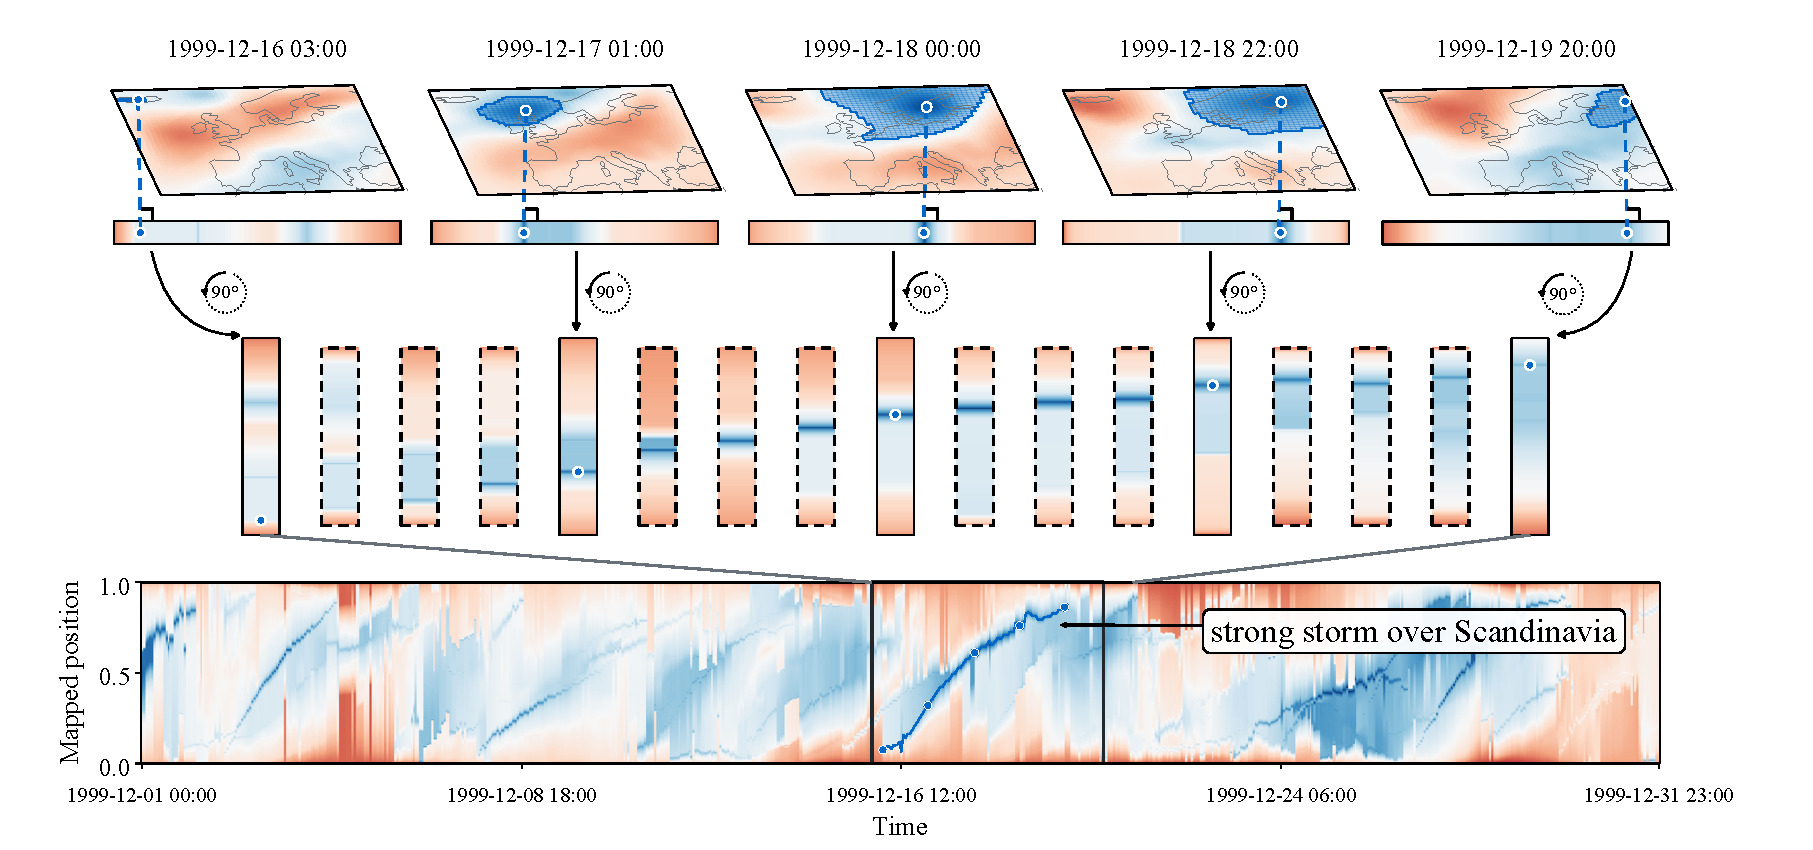
\includegraphics[width=\linewidth]{../figures/anchor_storms_overview.pdf}
\par
\refstepcounter{figure}\label{fig:storms_overview}
{\captionfonts\raggedright\noindent\figurename~\thefigure: Qualitative Storms archive ($\varepsilon=5\%$; preprocessing differs from Table~\ref{tab:quantitative-final}). Spatial snapshots and profiles identify one matched extremum; blue outlines show leaf-arc supports. Rotated profiles and dashed intermediate samples connect to its trajectory in the full 744-frame map.\par}

}
\linespread{0.90}
\setlength{\textfloatsep}{7pt}
\setlength{\floatsep}{6pt}
\setlength{\dbltextfloatsep}{7pt}
\begin{document}
\firstsection{Introduction}
\maketitle
\raggedbottom
\setlength{\emergencystretch}{1.5em}
An analyst who follows storms across an ocean or fire activity across a region reads a temporal overview for three things at once: which features exist and how they nest, where they are, and how they move. Animation keeps the spatial view of each instant but makes distant times hard to compare; static overviews give one display axis to time and compress space into the other~\cite{Tversky:2002:Animation,Robertson:2008:Animation,Bach:2017:STC}. What that second axis means decides which of these questions the overview can answer. Figure~\ref{fig:storms_overview} links the spatial supports of one feature to such a map.

Merge tree maps answer the first question well. Temporal Merge Tree Maps (TMTM) draw the merge tree of each frame as a 1D scalar profile and align the profiles along time, so minima show extrema and the barriers between them show merge levels~\cite{Koepp:2023:TMTM}. Spatiotemporal Merge Tree Maps (ST-MTM) add relative spatial distances and temporal position constraints to the layout~\cite{STMTM:2026}. Neither gives its display axis a fixed spatial meaning: TMTM orders leaves for the tree and for temporal alignment, and pairwise distances fix relative positions but no origin or direction. A feature's position therefore cannot be read as its longitude or its distance along a flow, and a feature that moves east need not move on the map. Hovm\"oller diagrams take the opposite side: they keep one physical coordinate and average the field over the others, so nearby extrema blend and the hierarchy disappears~\cite{Hovmoller:1949}.

Anchoring the axis means projecting every extremum onto one direction and placing it near its projection. The merge tree resists. An exact profile keeps every subtree in one contiguous block, but the projections of sibling subtrees can interleave. In Figure~\ref{fig:projection_conflict}, four minima project in the order $A,C,D,B$, which separates $A$ and $B$ by the $C,D$ subtree, so some features must leave their references or some merge levels must change; finite feature widths add packing constraints. ST-MTM observes that a one-dimensional layout cannot preserve all spatial distances, so some distortion is an expected consequence of the projection~\cite{STMTM:2026}. How much of it the hierarchy forces, where it arises and how much merge error buys it back have not been quantified, yet they decide whether a spatial axis is worth having.

We answer these questions. Three lower bounds give the displacement that exact topology, finite feature widths and a bounded merge error force on every admissible layout. They depend on the tree, the references and the widths, not on a solver, so the same computation measures any map, including TMTM and ST-MTM, and separates its error into a part forced by the hierarchy and a part chosen by its layout. A spatially anchored construction then builds maps that approach the bounds. It estimates one reference direction from matched extremum motion or takes one from the analyst, searches for a leaf order within a merge-error budget $\varepsilon$, sets optimal merge barriers, places anchors with a capped quadratic program and reconstructs the scalar profiles on a shared temporal axis. Exact Mode ($\varepsilon=0$) keeps the merge tree; Budgeted Mode ($\varepsilon>0$) trades a declared merge-level error for position.

Our main contributions are as follows:
\begin{itemize}
\setlength{\itemsep}{2pt}
\setlength{\parsep}{0pt}
\item a formulation of spatially anchored merge tree maps as hierarchy-constrained interval layouts with a fixed reference and a merge-level allowance, with three layout-independent lower bounds on the displacement that exact topology, finite widths and a bounded merge error force on any such layout, which locate each conflict and the merge error that releases it (Section~\ref{sec:bounds});
\item a spatially anchored construction with one primary control $\varepsilon$, built from a motion-derived reference, topology-budgeted leaf ordering, optimal merge barriers and capped spatiotemporal anchor placement (Sections~\ref{sec:reference} and~\ref{sec:construction});
\item an evaluation showing that the bounds are attained on controlled trees and by the selected order on 606 of 614 planar frames, that 31--95\% of the order error of TMTM and ST-MTM is not forced by the tree, and that the anchored maps place features much closer to their references than TMTM and ST-MTM on the four planar sequences of the ST-MTM benchmark and two volumetric flows, within every declared merge budget (Section~\ref{sec:experiments}).
\end{itemize}

% Former Figure 2 temporarily removed; source retained in figures/source/ring_result_20261106.


\section{Related Work}\label{sec:related}
\subsection{Spatially Referenced Temporal Visualization}
Static temporal displays expose distant observations simultaneously, while animation retains the spatial view of each instant; their usefulness depends on the analytical task~\cite{Tversky:2002:Animation,Robertson:2008:Animation}. Generalized space--time cubes describe the transformations connecting such views~\cite{Bach:2017:STC}. In compressed temporal overviews, the spatial coordinate determines which location and motion relationships remain directly interpretable.

Hovm\"oller diagrams retain a selected physical coordinate and summarize the other dimensions~\cite{Hovmoller:1949}. Geographic orderings and space-filling curves instead traverse the domain~\cite{Guo:2006:SpatialOrder,Dafner:2000:CSFC}. Dynamic Volume Lines and data-driven curves extend spatial traversal to volumetric comparison and scalar-aware ordering~\cite{Weissenboeck:2019:DVL,Zhou:2021:DSF}. A traversal can retain spatial neighborhoods, but its 1D coordinate is generally different from a fixed projection, and traversal adjacency alone does not enforce the merge hierarchy.

1D projections organize spatiotemporal phenomena~\cite{Franke:2021:1DP}, and MotionRugs expose collective behavior of moving entities~\cite{Buchmueller:2019:MR}. More generally, an embedding trades original-domain relationships against its display organization~\cite{Nonato:2019:MP}. Relative proximity does not determine an absolute coordinate. We assign fixed projection targets to topological features and bound their displacement under hierarchical and interval constraints for any layout, combining spatial reference with a temporal topology overview.

\subsection{Topology-Based Temporal Maps and Geometry-Aware Layouts}
Topology-based visualization organizes scalar structures through connectivity~\cite{Heine:2016:Survey}. Landscapes and landscape profiles express hierarchies through terrain or 1D scalar representations~\cite{Weber:2007:TL,Oesterling:2013:TLP}, with geometry-preserving and temporally coherent extensions~\cite{Beketayev:2012:GPTL,Herick:2020:TCTL}. These representations connect scalar values and feature relationships in a compact view.

TMTM emphasizes intact topological features and temporal alignment in static merge-tree maps~\cite{Koepp:2023:TMTM}. ST-MTM incorporates relative spatial geometry and temporal position constraints~\cite{STMTM:2026}. These priorities give spatial relationships and coherence a role in the map, while leaving its display coordinate free to differ from a fixed physical direction. We estimate a shared direction from extremum motion, or accept a physical direction, and couple that reference to topology-budgeted layout and to position bounds that hold for any layout. The construction reuses the established profile and scalar-filling foundation.



Hierarchy-constrained leaf ordering traditionally minimizes adjacent dissimilarity~\cite{BarJoseph:2001:OLO}; target-order reordering studies related tree-consistent permutations~\cite{Bulteau:2022:RT}. Separation-constrained layouts control geometric overlap and displacement~\cite{Dwyer:2006:IPSEP,Li:2019:SOI}. We couple these layout concerns to fixed spatial targets and bound the displacement they force. Its exact-topology point-order bound has a closed form, whereas finite-width candidate ordering remains heuristic.

Merge-tree comparison depends on the descriptors and correspondences used~\cite{Yan:2021:Survey}. Labelled cophenetic/interleaving comparisons support fixed-identity merge-level accounting~\cite{Munch:2019:LINF,Gasparovic:2024:IID}, and ordered merge trees connect scalar curves to monotone interleaving distances~\cite{Beurskens:2025:OMT}. We use fixed labels to measure displayed merge error. The optimal-barrier subproblem relates to minimax ultrametric fitting~\cite{Farach:1995:RM}, with the additional restriction that one linear order induces every displayed merge.

\begin{figure*}[t]
\centering
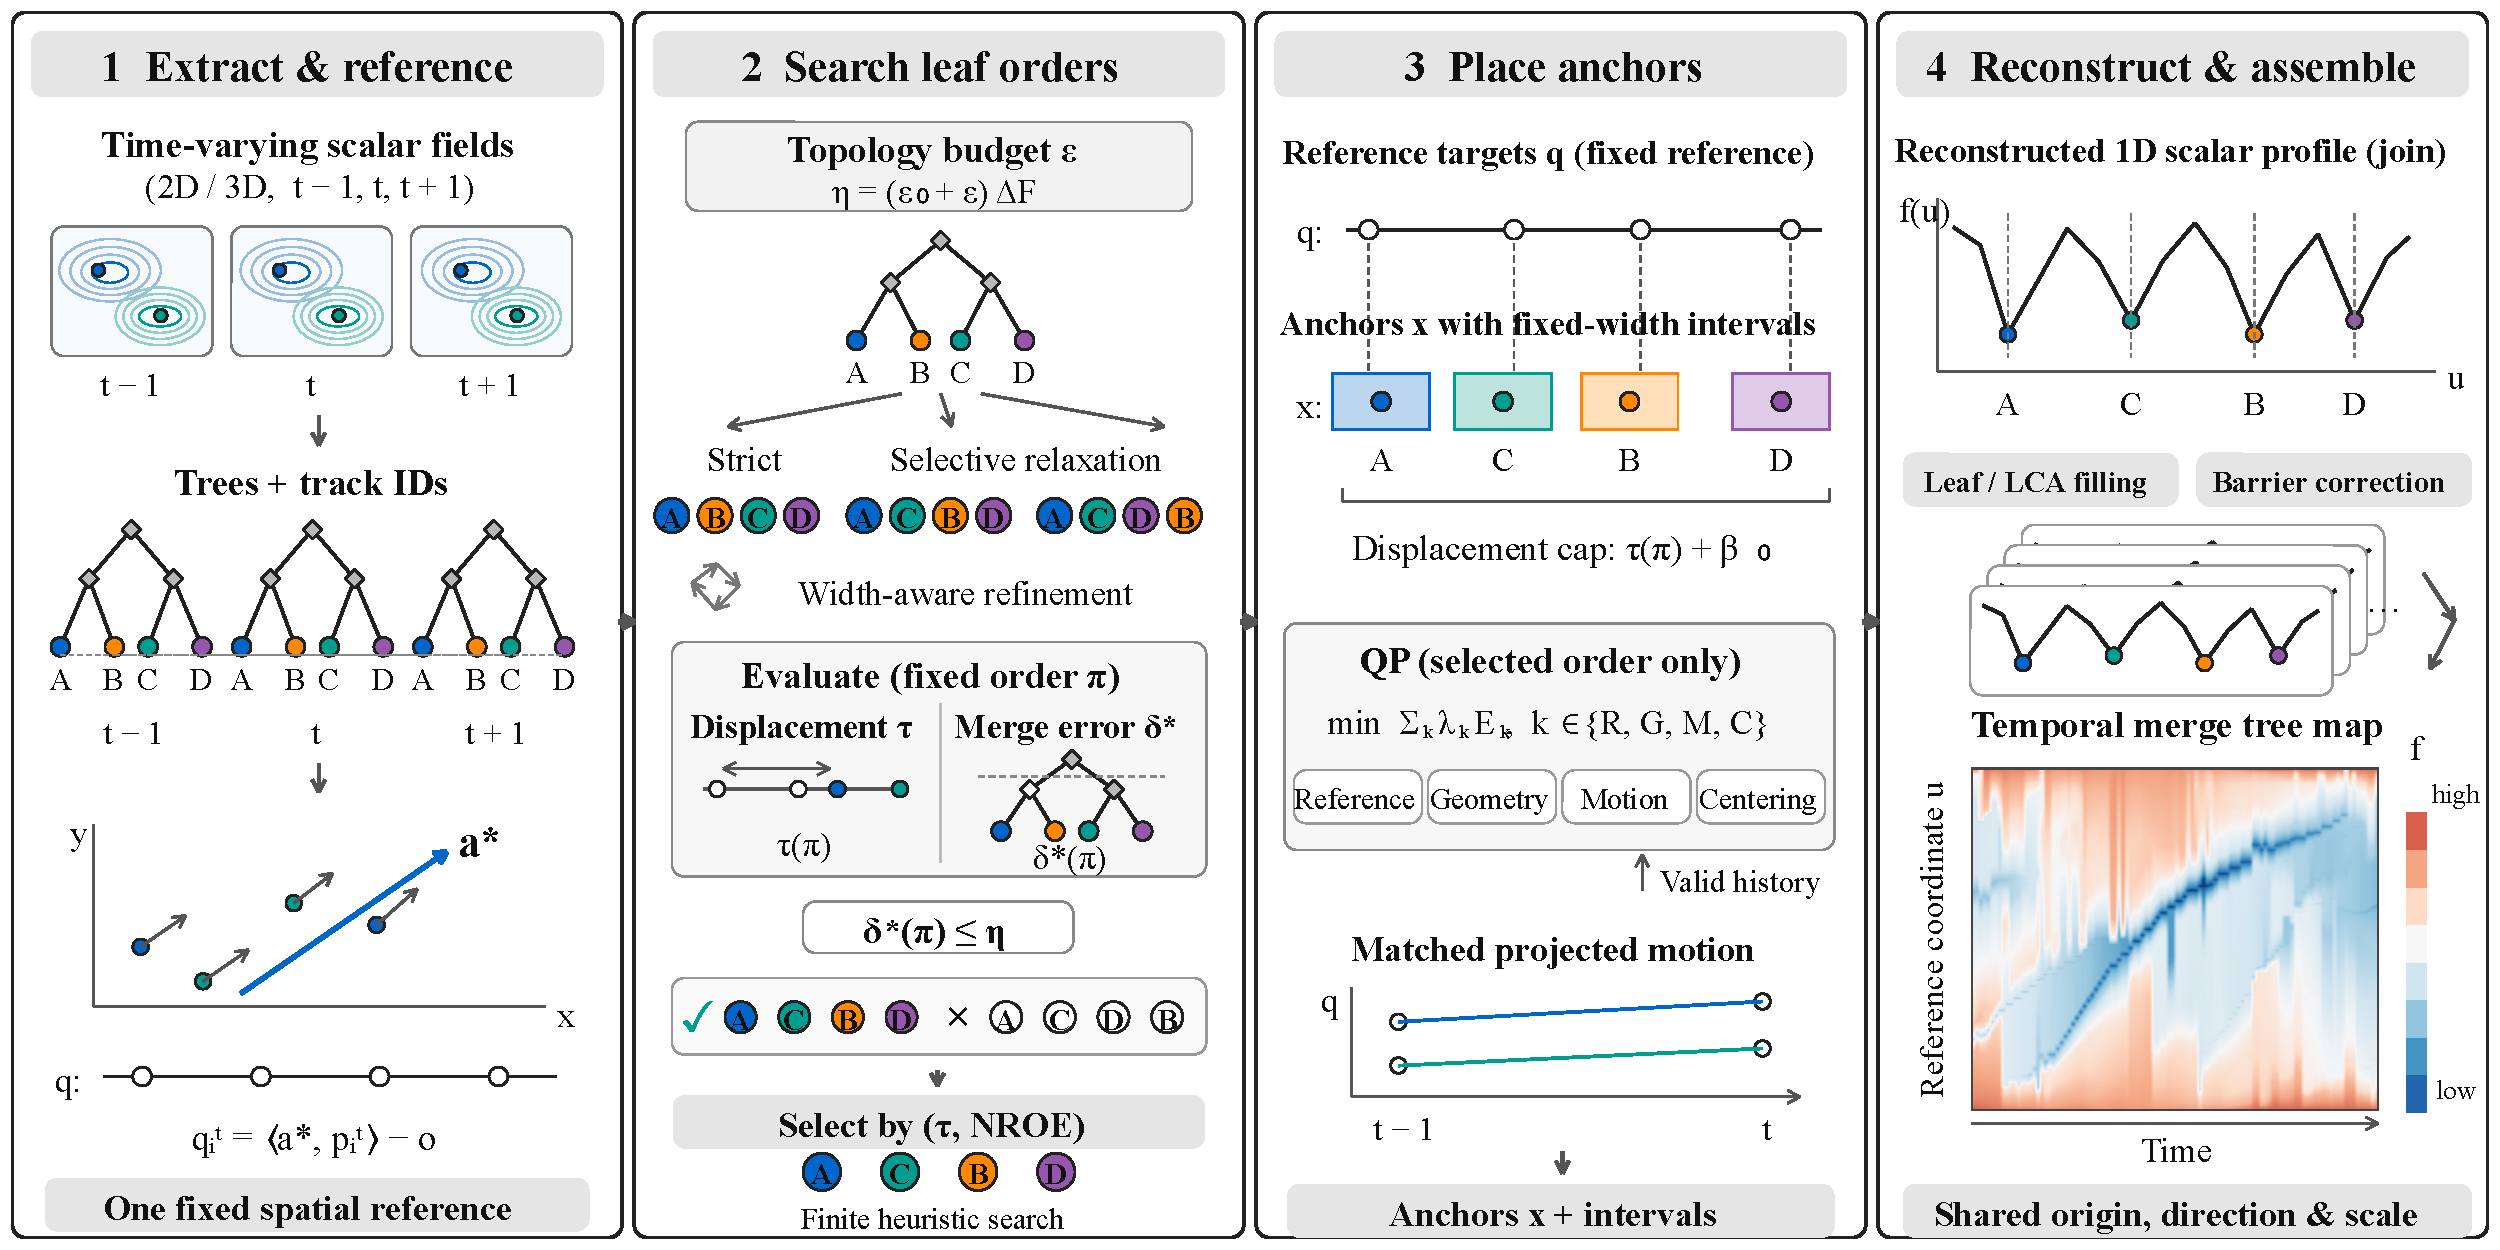
\includegraphics[width=\textwidth]{../figures/anchor_framework.pdf}
\caption{Anchored construction. (1) Extract augmented merge trees and match leaf supports, then estimate one fixed spatial reference from matched extremum motion. (2) Refine candidate leaf orders, admit those satisfying the merge-error allowance, and select by fixed-order displacement and NROE. (3) Optimize anchors within nonoverlapping intervals under a displacement cap, using valid matched history. (4) Reconstruct scalar profiles with barrier correction and assemble the temporal map. Diagrams are schematic; the map is an existing qualitative Storms output at $\varepsilon=10\%$. Order search is heuristic, and continuous feasibility and rendered errors are checked separately.}
\label{fig:framework}
\end{figure*}





\section{Background}\label{sec:background}
\subsection{Augmented Merge Trees and Feature Supports}
For a sampled 2D or 3D field $f_t:D\to\mathbb{R}$, the merge tree $T_t$ records sublevel-set connectivity: minima create components and saddles join them as the threshold increases. Negating the field gives the split-tree convention. Critical points are supernodes connected by superarcs; augmentation associates regular vertices with these arcs~\cite{Koepp:2023:TMTM,STMTM:2026,Tierny:2018:TTK}. Extraction and simplification precede layout.

A leaf represents an extremum at spatial location $p_i^t$. Its feature support $S_i^t$ consists of that extremum and the regular samples on its incident leaf arc, excluding the parent critical sample. It is not the full component or the complete subtree above that arc. For cross-frame overlap, these supports are sets of stable spatial sample IDs: the same ID must denote the same spatial sample across frames. Fixed-grid inputs preserve this identity through consistent sample indexing. Internal arcs retain further regular samples for scalar filling. Write $\mathcal{D}_t(v)$ for the descendant leaf labels of a node $v$, and $h_t(v)$ for its scalar level. The lowest common ancestor determines the merge-height matrix:
\begin{equation}\label{eq:merge}
 V_{ij}^t=h_t(\lca(i,j)),\quad i\ne j;\qquad
 V_{ii}^t=f_t(p_i^t).
\end{equation}
Equal-level merge events form one multifurcation; arbitrary binary refinements do not add strict constraints. All subsequent guarantees refer to the supplied, possibly simplified tree.

\subsection{One-Dimensional Merge-Tree Profiles}
A 1D merge-tree profile represents extrema at anchors in a selected leaf order. Regular vertices on leaf arcs supply scalar context within leaf intervals; internal arcs and paths to the LCA supply the intervening gaps~\cite{Koepp:2023:TMTM,STMTM:2026}. In join convention, extrema become profile minima, and the largest profile value between two anchors gives their displayed merge level. Exact preservation requires each strict subtree to occupy a contiguous leaf block. Arranging these profiles along time yields a static temporal map. This profile model provides the basis for the spatial anchoring formulation below.




\section{Spatially Anchored Maps}\label{sec:method}
Figure~\ref{fig:framework} summarizes the construction. It connects a shared spatial reference to the displayed leaf anchors. We construct the reference and formulate the layout, describe the construction, and then explain its unavoidable position costs through certified bounds. Analysis uses join convention; split-tree scalar signs are restored after reconstruction.

\subsection{Spatial Reference and Problem Formulation}\label{sec:reference}
\paragraph{Cross-frame Leaf Correspondence.}
We track merge-tree leaf extrema $p_i^t$ using their leaf-arc supports $S_i^t$. On a shared fixed grid, overlap-based preprocessing~\cite{STMTM:2026} counts common spatial samples:
\begin{equation}\label{eq:overlap}
 O_{ij}^t=|S_i^t\cap S_j^{t+1}|.
\end{equation}
Hungarian assignment maximizes total intersection count over one-to-one pairs, discarding zero-overlap pairs. The assigned links define the identity states described below.

\emph{Continuation} inherits a Track ID; \emph{birth/death} starts an unmatched current identity or ends an unmatched previous track. For \emph{non-bijective correspondence}, including potential one-to-many, many-to-one and ambiguous relations, only the assigned one-to-one links are retained. These identity states neither identify physical split/merge events nor form a branching lineage. For a current leaf $i$, $\mu_t(i)$ denotes its valid predecessor. The layout receives precomputed tracks aligned to leaf rows; upstream support and confidence conventions are detailed in Supplementary Material.

% Previous correspondence figure temporarily removed; source preserved in figures/source/open_mechanisms_20261106/.

These correspondences, computed before any topology-budget sweep, provide the motion samples for Spatial Anchoring, which distinguishes a reference target $q_i^t$ from the display anchor $x_i^t$. Only valid consecutive-frame matches contribute displacements; failed matches or interrupted tracks contribute no sample for that step. By default, one unit direction $a^*\in\mathbb{R}^d$, $d\in\{2,3\}$, is estimated offline from all matched consecutive-frame extremum displacements:
\begin{equation}\label{eq:autodirection}
\begin{aligned}
 \Delta p_i^t&=p_i^t-p_{\mu_t(i)}^{t-1},\\
 S&=\sum_{t,i\;\mathrm{matched}}\Delta p_i^t(\Delta p_i^t)^\top,\\
 a^*&\in\arg\max_{\|a\|=1}a^\top Sa.
\end{aligned}
\end{equation}
The leading eigenvector maximizes squared projected motion, not feature count or topological compatibility. The same calculation serves 2D and 3D; it is performed once for the whole sequence. Its sign makes total signed projected motion nonnegative; for near-zero signed motion, the largest-magnitude component is made positive. With negligible motion energy, the longest domain axis is used (first axis on a tie). Repeated leading eigenvalues leave the maximizing direction nonunique; the reported eigengap indicates this ambiguity. A supplied physical direction may replace $a^*$ without changing the layout. Overlap matching may miss fast-moving features or those with changing or weakly overlapping supports, affecting the displacement sample and hence the estimated direction.



\begin{figure}[t]
\centering
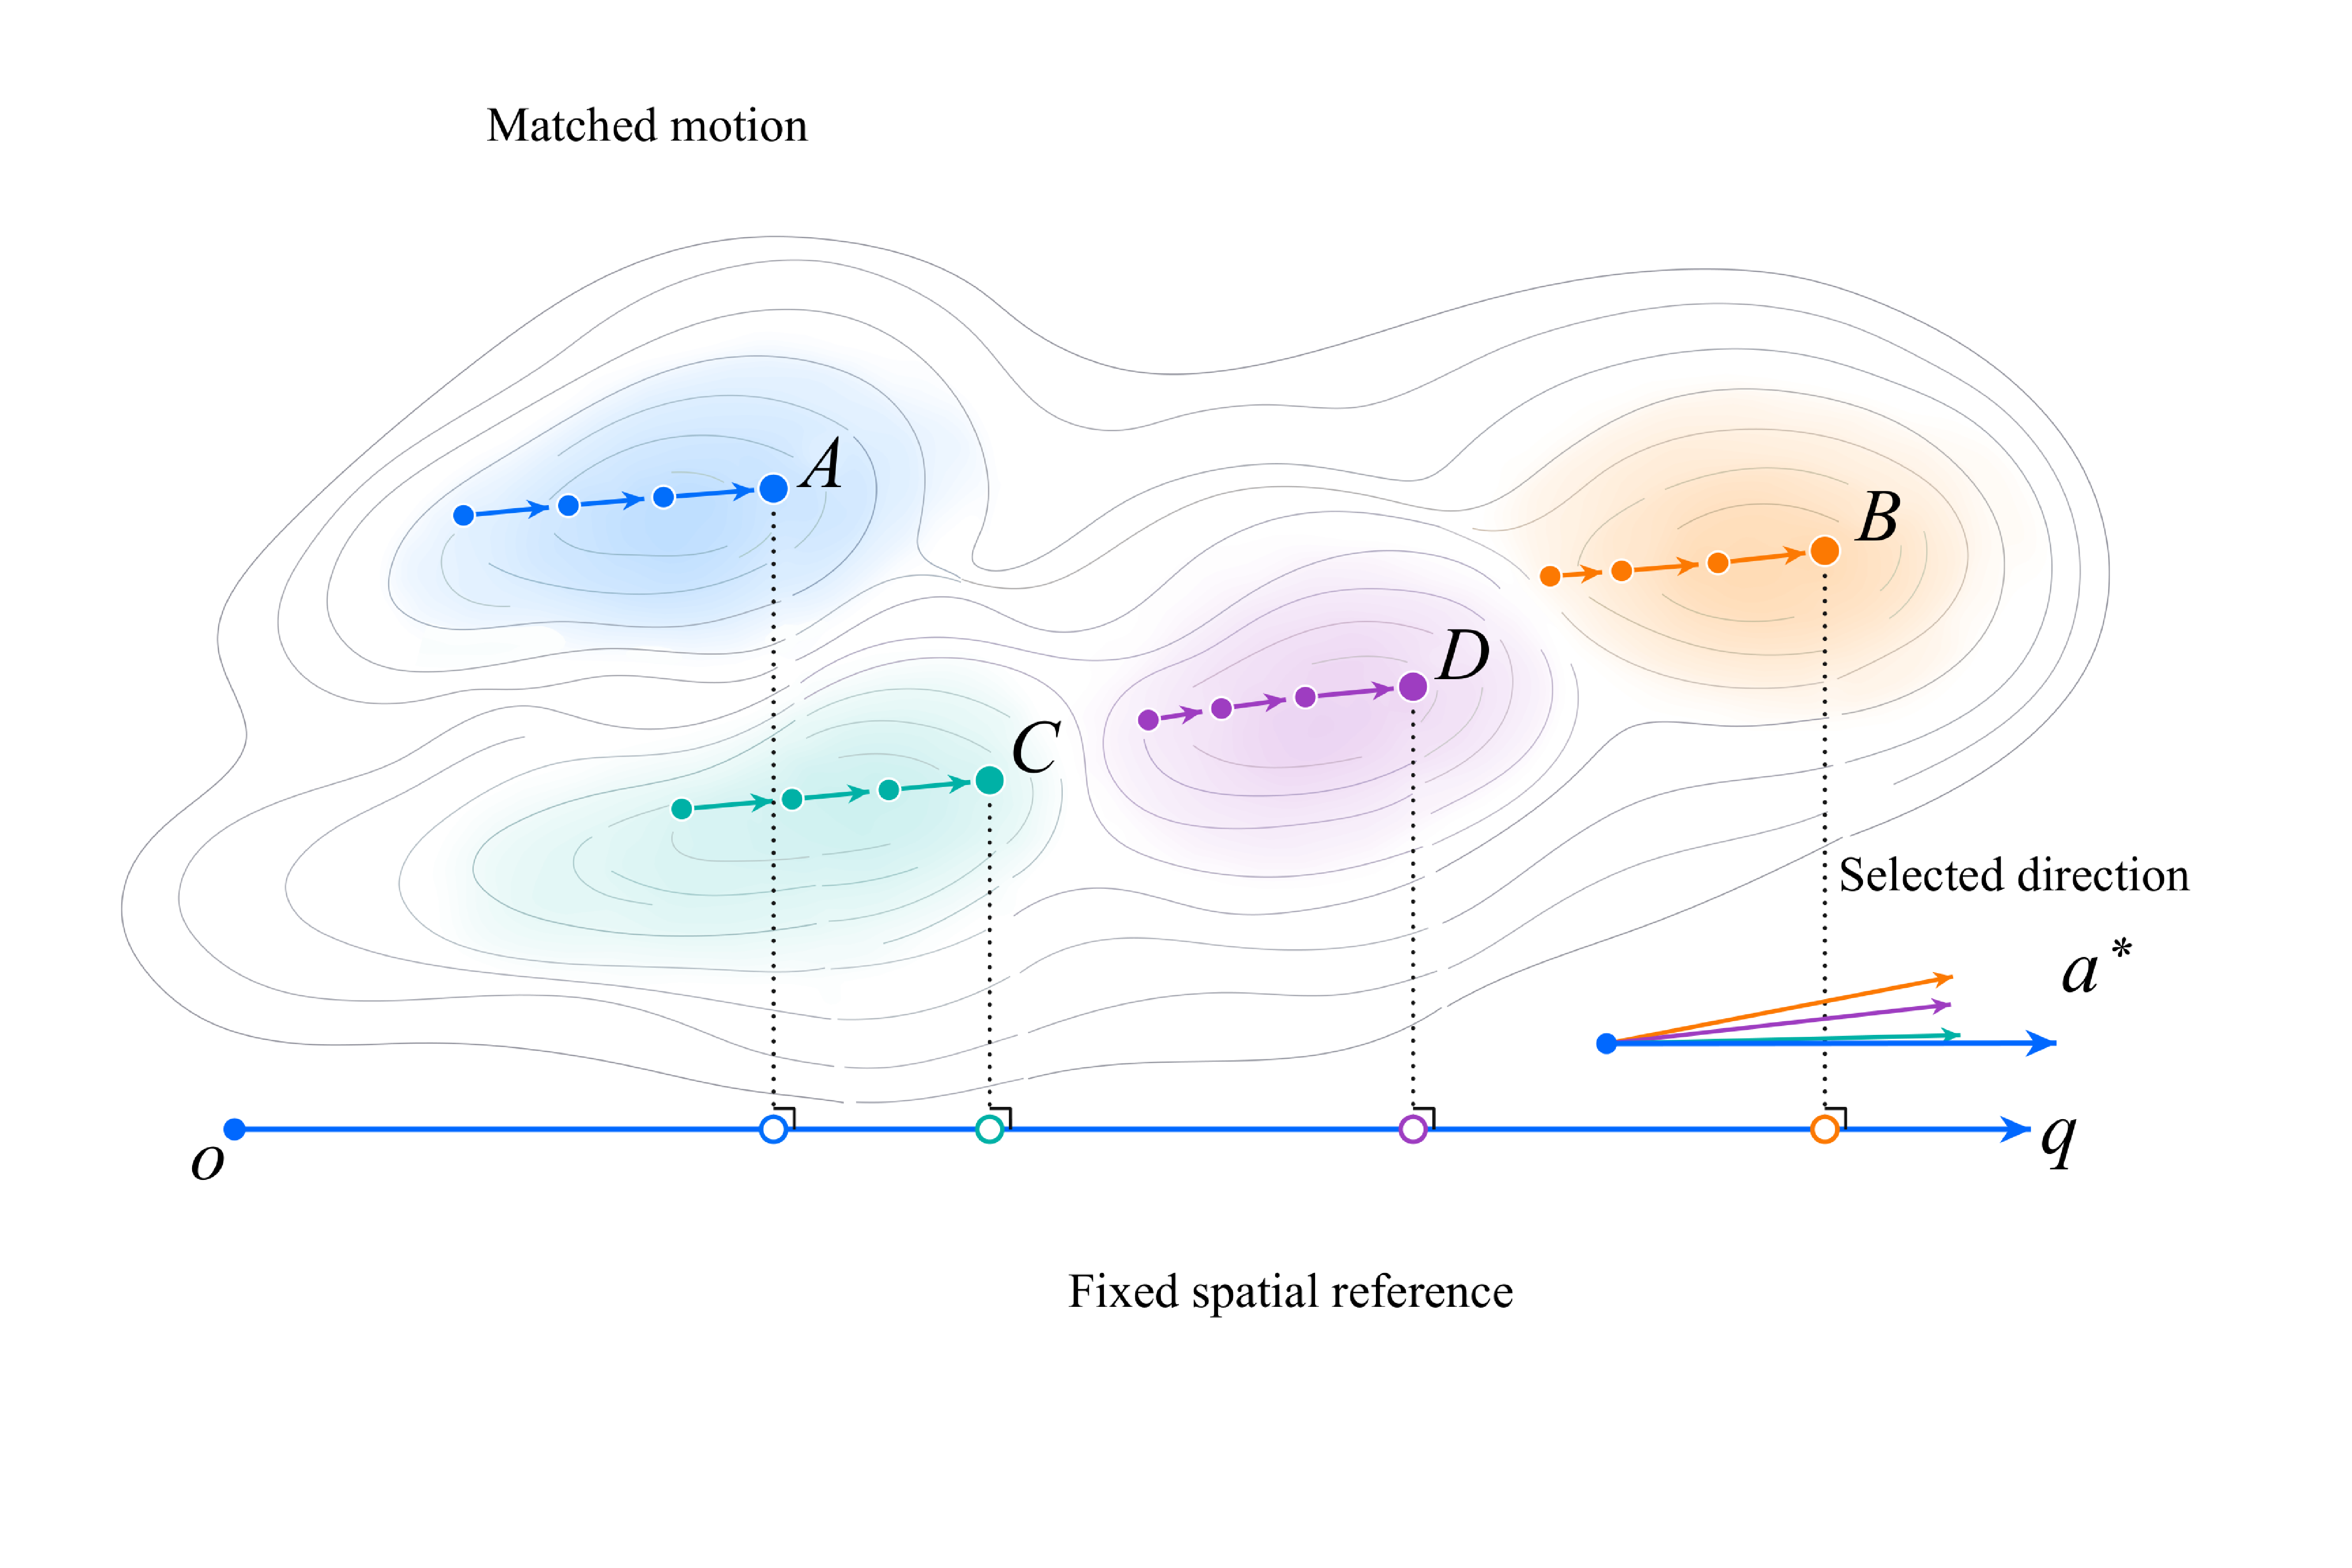
\includegraphics[width=0.85\columnwidth]{../figures/anchor_direction_open.pdf}
\caption{Motion-derived spatial reference. Matched extremum displacements define one direction $a^*$ for the sequence; extrema project onto the parallel reference axis $q$ from a common origin $o$. Tracks, contours and projection positions are schematic.}
\label{fig:direction-open}
\end{figure}
Figure~\ref{fig:direction-open} illustrates the shared reference. For the selected direction, the minimum and span of the projected domain bounding-box corners define a common origin $o$ and extent $L>0$. The reference is
\begin{equation}\label{eq:reference}
 q_i^t=\langle a^*,p_i^t\rangle-o\in[0,L].
\end{equation}
Direction, origin and scale remain fixed across frames and all budgets for the same prepared sequence. Distinct extrema can share projected coordinates while retaining separate identities. Anchoring minimizes constrained deviation rather than requiring $x_i^t=q_i^t$.

Relative geometry uses distances $d_{ij}^t$ between leaf-support centroids. These differ from extremum references because a changing support can move its centroid while the extremum stays fixed. The automatic-reference adapter supplies extrema explicitly; the low-level solver also accepts precomputed references and otherwise defaults to centroid projection. Widths $W_i^t=s\,m_i^t$ convert positive support measures with a fixed scale $s$, without per-frame normalization.

Figure~\ref{fig:projection_conflict} contrasts the spatial target order with a tree-consistent order. In this four-minimum example, projected order $A,C,D,B$ separates $A$ and $B$ by the $C,D$ subtree, violating the required contiguity of $\{A,B\}$; exact topology therefore cannot realize all four targets without displacement.



With correspondence and the reference fixed, a frame comprises a leaf order, extremum anchors, and a scalar profile:
\begin{equation}\label{eq:mapframe}
 M_t=(\pi_t,x_t,\psi_t),\qquad\psi_t:[0,L]\to\mathbb{R}.
\end{equation}
We seek reference-aligned positions and motion while approximating relative geometry and controlling displayed topology. The interval-layout set $\mathcal{L}(\pi)$ requires intervals of widths $W_i$ centered at $z_i$ to lie inside the canvas, remain disjoint with gap at least $g\ge0$, and contain anchors satisfying $|x_i-z_i|\le\rho W_i/2$, $0\le\rho\le1$. Infeasible total widths and gaps are reported rather than rescaled.

Actual displacement is $|x_i-q_i|$, normalized by $L$ when reported. To distinguish order conflict from finite-width placement, define
\begin{equation}\label{eq:nroe}
 \nroe(\pi)=\frac{1}{2L}\max_{j\le k}
                      [q_{\pi(j)}-q_{\pi(k)}]^+.
\end{equation}
This is the smallest worst displacement of a nondecreasing point placement, divided by $L$; it ignores widths. For finite intervals, the exact fixed-order cost is
\begin{equation}\label{eq:tau}
 \tau(\pi)=\min_{(x,z)\in\mathcal{L}(\pi)}\|x-q\|_\infty.
\end{equation}
The minimum is attained whenever the layout set is nonempty. It is evaluated exactly from the fixed-order packing constraints, equivalently through a minimax linear program.

For distinct labels, let $V_{ij}^{\psi}$ be the maximum profile value between their anchors, with $V_{ii}^{\psi}=\psi(x_i)$. We require
\begin{equation}\label{eq:dtop}
\begin{aligned}
 \dtop(\psi_t,T_t)&=\max_{i,j}|V_{ij}^{\psi_t}-V_{ij}^t|\le\eta,\\
 \eta&=(\varepsilon_0+\varepsilon)\Delta_F.
\end{aligned}
\end{equation}
Here $\Delta_F>0$ is the sequence-wide scalar range, $\varepsilon_0$ is a fixed numerical allowance, and $\varepsilon\ge0$ is the sole primary user control. The implementation defaults to $\varepsilon_0=10^{-7}$. NMLE reports the achieved normalized error $\dtop/\Delta_F$. Exact topology means zero labelled error on the declared tree. A nonzero tie allowance is accounted for in $\eta$.

All remaining settings belong to a fixed configuration $\Theta_0$: position slack $\beta_0$, the four objective weights, width scale, gap, anchor slack and output resolution. For a prepared sequence, the default interface is $M_t^\varepsilon=\mathcal{A}(T_t,q_t,W_t,V_t,\mu_t;\varepsilon,\Theta_0)$. Advanced settings may be supplied once, but only $\varepsilon$ varies in a budget sweep. Supplementary Material specifies the fixed scale rules and implementation tolerances.

For canonical cophenetic merge-tree representations whose fixed labels cover every leaf and whose induced matrices include the diagonal, $\dtop$ equals the unnormalized labelled interleaving distance~\cite{Munch:2019:LINF,Gasparovic:2024:IID}. Under these conditions, $d_B\le d_I\le\dtop$~\cite{Morozov:2013:IDMT}. Unlabelled extrema introduced by rendering must be checked before applying this interpretation to the whole displayed tree.

\begin{figure}[t]
\centering
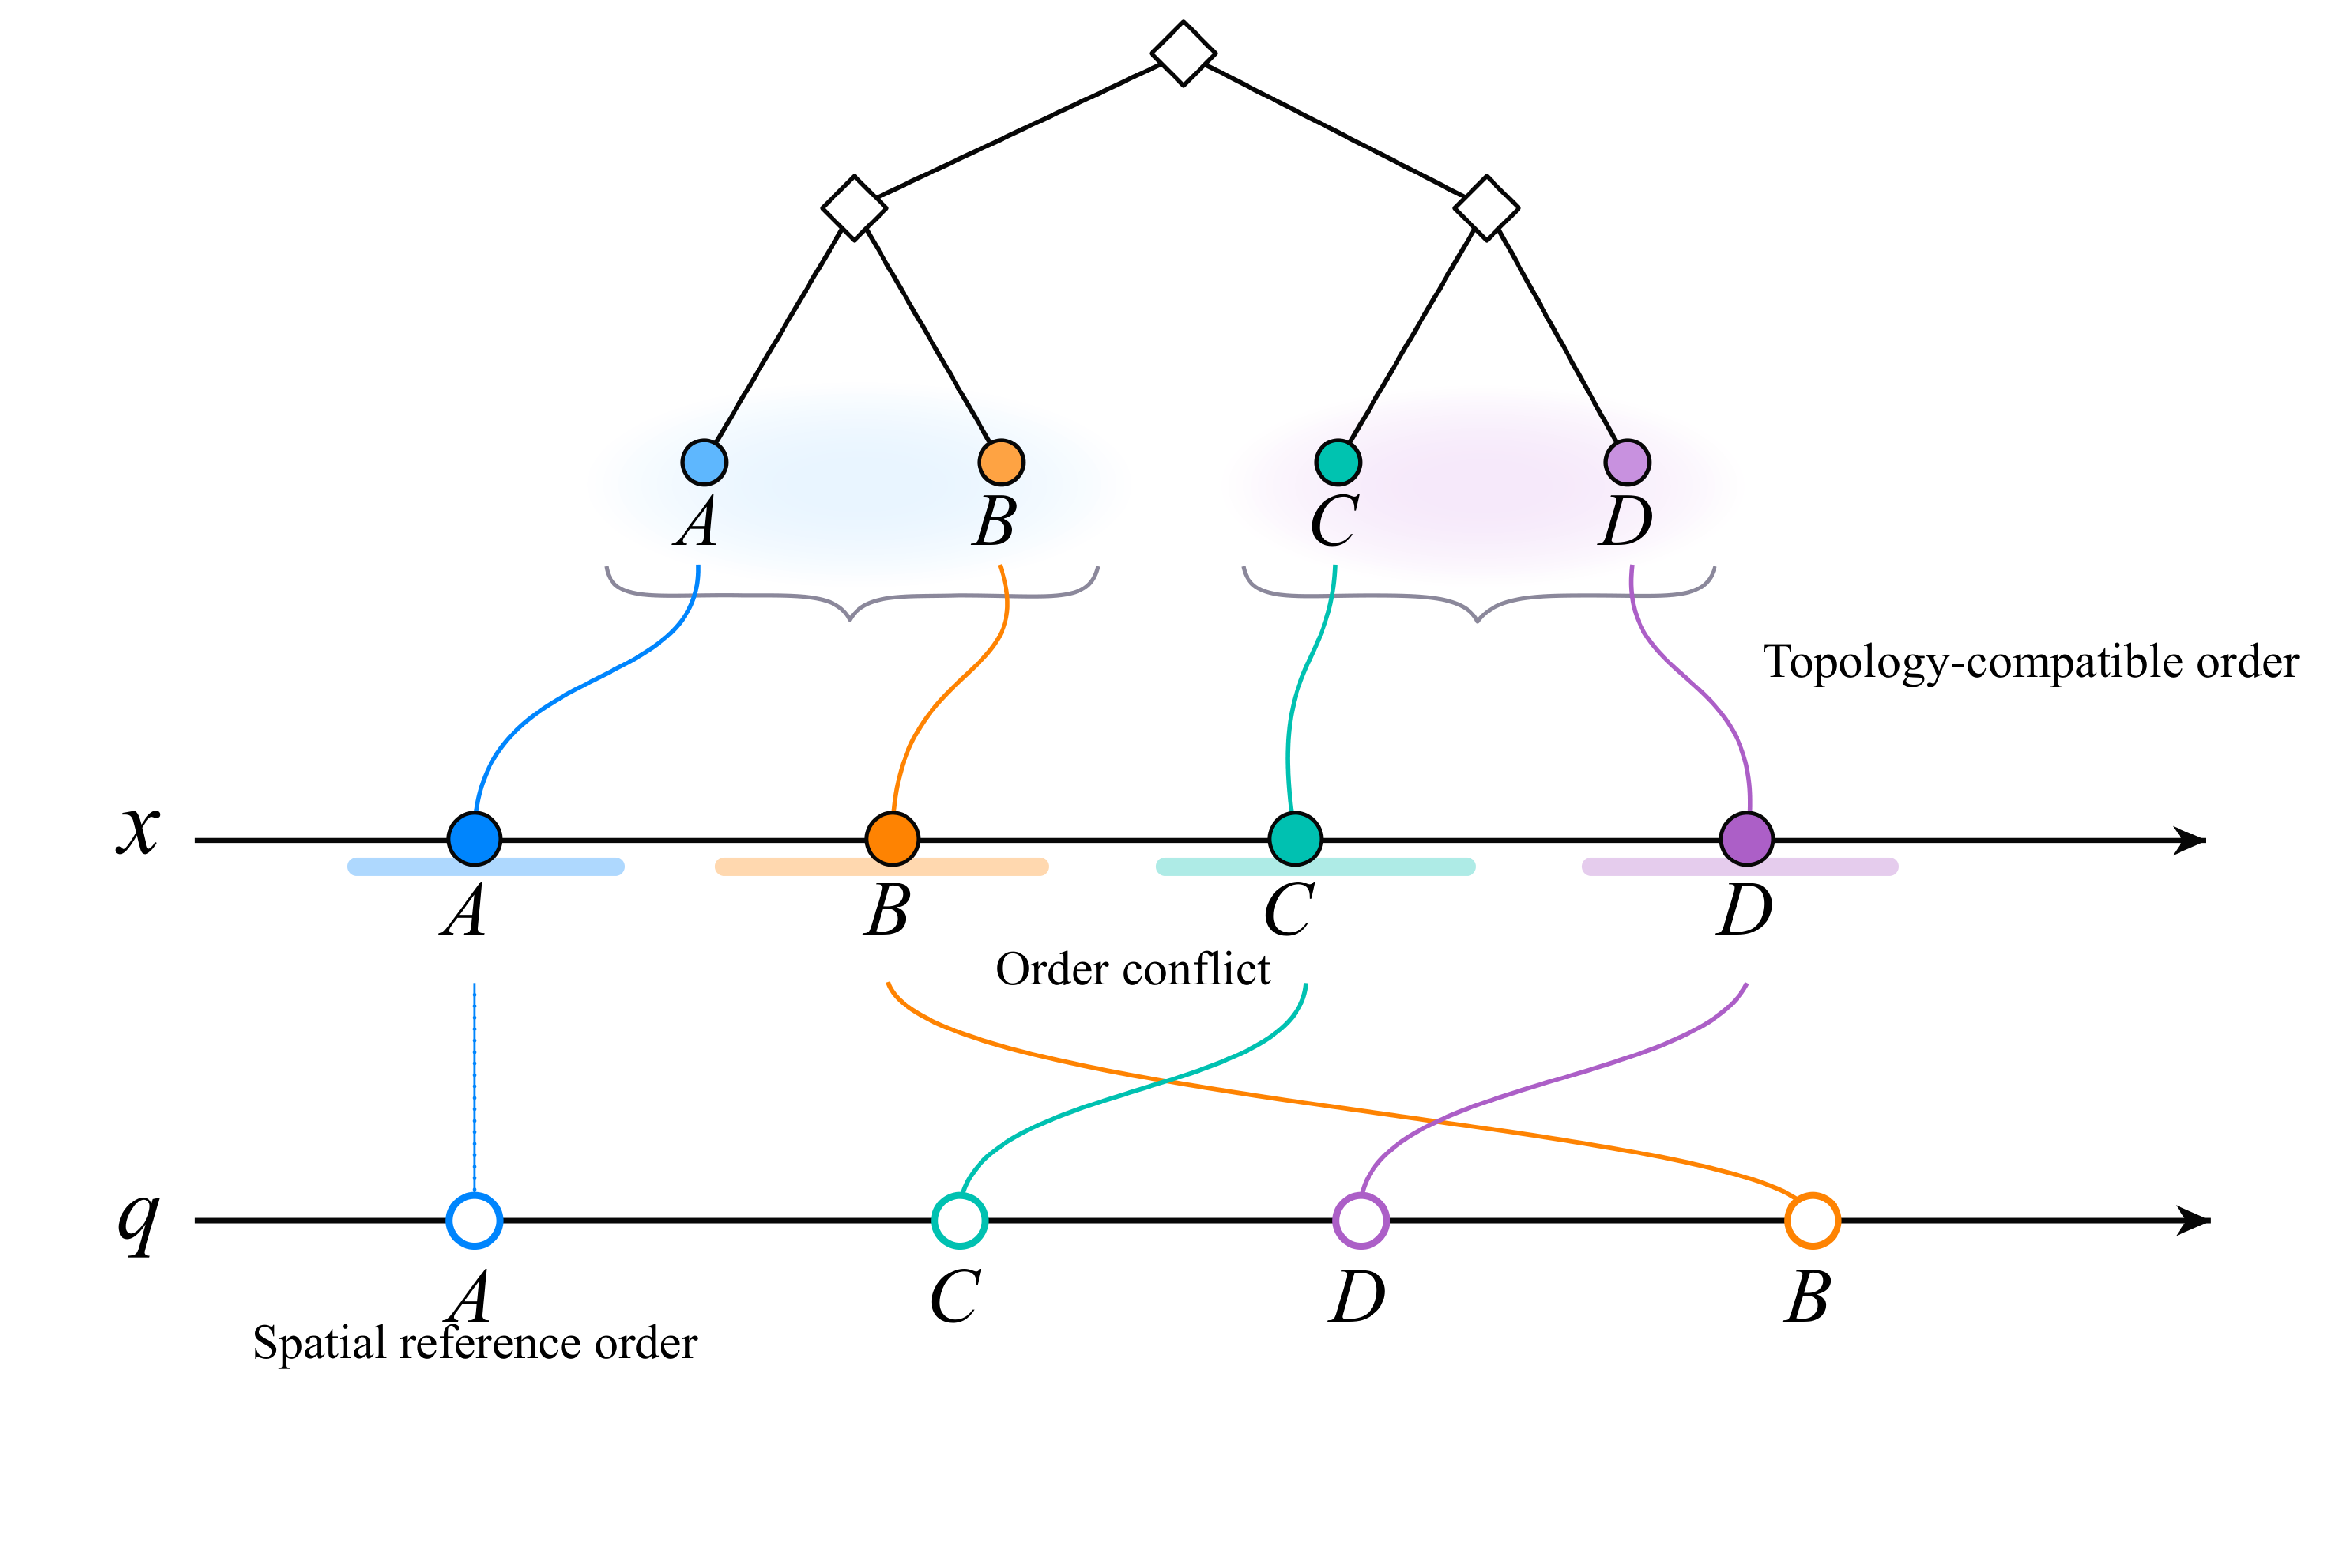
\includegraphics[width=\columnwidth]{../figures/anchor_conflict_open.pdf}
\caption{Reference--topology conflict. The tree requires contiguous $A,B$ and $C,D$ blocks. Its displayed anchors $x$ follow a compatible order, whereas the fixed spatial targets $q$ occur as $A,C,D,B$. Colored links indicate the displacement needed to reconcile these orders. Widths and positions are schematic.}
\label{fig:projection_conflict}
\end{figure}
\subsection{Spatially Anchored Layout Construction}\label{sec:construction}
With features and their reference fixed, construction chooses an order by the lexicographic objective
\begin{equation}\label{eq:orderobjective}
\begin{aligned}
 \pi_t^\varepsilon&\in\underset{\pi\in\mathcal{C}_t(\varepsilon)}{\arg\min}
                    \bigl(\tau_t(\pi),\nroe_t(\pi)\bigr),\\
 &\hspace{1em}\mathrm{s.t.}\quad\delta_t^*(\pi)\le\eta(\varepsilon).
\end{aligned}
\end{equation}
The finite candidate pool contains the original strict-topology order, midpoint initializations, and orders visited during width-aware refinement of threshold and selective flattenings. Every candidate is evaluated against the same source merge matrix. Selection minimizes $\tau$ first and NROE second; it is not a global optimum over all permutations. Algorithm~\ref{alg:construction} separates this discrete selection from fixed-order placement.

\begin{algorithm}[htbp]
\caption{Single-control anchored construction}\label{alg:construction}
\KwData{2D/3D field sequence and grid; $\varepsilon\ge0$; fixed configuration $\Theta_0$.}
\KwResult{Temporal map $I^\varepsilon$, error records, or a failure report.}
Extract augmented trees, leaf supports and extrema; match supports and assign Track IDs\;
Estimate one direction and fixed references $q_t$; reuse this preprocessing across budgets\;
$\eta\leftarrow(\varepsilon_0+\varepsilon)\Delta_F$\;
\For{each time step $t$ in temporal order}{
 Report and stop if widths and gaps exceed the fixed canvas\;
 $\mathcal{C}_t\leftarrow\operatorname{GenerateAndRefine}(T_t,q_t,W_t,V_t,\eta)$; retain strict-topology candidates\;
 Evaluate $\tau(\pi)$, $\nroe(\pi)$ and $\delta^*(\pi)$ for candidates\;
 $\mathcal{F}_t\leftarrow\{\pi\in\mathcal{C}_t:\delta^*(\pi)\le\eta\}$\;
 \lIf{$\mathcal{F}_t=\varnothing$}{report no feasible candidate and stop}
 Select $\pi_t^\varepsilon$ from $\mathcal{F}_t$ by $(\tau,\nroe)$\;
 Compute optimal merge barriers for $\pi_t^\varepsilon$\;
 Solve the four-term QP only for $\pi_t^\varepsilon$, with cap $\tau(\pi_t^\varepsilon)+\beta_0$ and valid matched history\;
 Reconstruct the profile by leaf/LCA filling and barrier correction\;
 Record candidate counts, continuous and rendered errors, motion and failures; append profile to $I^\varepsilon$\;
}
\KwReturn{$I^\varepsilon$ and diagnostic records}\;
\end{algorithm}

\subsubsection{Topology-Budgeted Leaf Ordering}
\emph{Exact Mode} sets $\varepsilon=0$, leaving only the numerical allowance $\eta=\varepsilon_0\Delta_F$, which merges saddles tied to within $\varepsilon_0\Delta_F$; strict exact topology is $\eta=0$. \emph{Budgeted Mode} permits $\varepsilon>0$. Both modes share the same interval model and placement objective.

Candidate generation includes the exact tree, threshold flattenings, and a conflict-driven selective flattening. Midpoint orders initialize these structures. Width-aware block insertion refines the four best initial structures, together with the exact tree, while retaining the point-model budget order as a candidate. Moves improve the lexicographic score consisting of $\tau$ and a squared packing-residual term, and must pass $\delta^*(\pi)\le\eta$. Visited initial and trial orders are retained in the deduplicated pool, including the strict-tree initialization and retained point candidate. Final budget filtering and lexicographic selection use the exact fixed-order costs; refinement does not certify a global optimum over permutations. 

Figure~\ref{fig:selective_relaxation} illustrates the additional ordering freedom created by a selective flattening. Removing the $A$--$B$ sibling constraint admits the order $A,C,D,B$ while retaining the $C$--$D$ subtree. This structural proposal still requires evaluation against the original merge matrix and the prescribed error budget.



Helpers inherit the current geometry and layout parameters. Comparisons use the implementation's numerical tolerances. The guards report capacity failure or an empty admitted set; no widths, gaps or canvas scales are silently changed. The exact-tree structure is always retained among refinement seeds, and its child-block moves preserve strict topology in the exact model. Its presence does not guarantee successful numerical placement or raster reconstruction; capacity, input and solver failures remain possible. An empty admitted set is never selected from. Invalid input and numerical solver failures propagate as errors, separately from mathematical infeasibility. First-frame and unmatched history contributes no temporal target.

\subsubsection{Optimal Merge Barriers and Topological Feasibility}
For a fixed order, a pair's displayed merge is the largest intervening barrier. Set $C_k=\min_{i\le k<j}V_{\pi(i)\pi(j)}$ and $F_k=\max(V_{\pi(k)\pi(k)},V_{\pi(k+1)\pi(k+1)})$ for gap $k$.
\begin{proposition}[Optimal barriers]\label{prop:barriers}
With fixed extremum values in the continuous non-strict model, the smallest labelled merge error is
\begin{equation}\label{eq:delta}
\begin{split}
 \delta^*(\pi)=\max\bigg\{&0,\max_k(F_k-C_k),\\
 &\frac12\max_{i<j}\left(V_{\pi(i)\pi(j)}-
                         \max_{i\le k<j}C_k\right)\bigg\},
\end{split}
\end{equation}
and barriers $b_k=C_k+\delta^*(\pi)$ attain it.
\end{proposition}
Error $\delta$ requires $F_k\le b_k\le C_k+\delta$. Choosing the largest admissible barriers satisfies every pair's lower merge requirement exactly when $\delta\ge\delta^*$. Thus the order meets the merge-level allowance in this continuous model exactly when $\delta^*(\pi)\le\eta$. This fixed-order test supports candidate search without making it globally optimal. Strict-extremum clearance and raster effects are checked separately.

\subsubsection{Spatially Anchored Spatiotemporal Placement}
Once the order is fixed, the core terms are $E_R$, mean squared deviation from the fixed reference, and $E_M$, mean squared error in matched projected motion. The auxiliary term $E_G$ approximates support-centroid distances through ordered anchor separations; $E_C$ regularizes anchor offsets from interval centers. All four terms and their nonnegative weights are retained:
\begin{equation}\label{eq:qp}
\begin{aligned}
 \min_{x_t,z_t}\quad&\lambda_R E_R+\lambda_G E_G+\lambda_M E_M+\lambda_C E_C\\
 \mathrm{s.t.}\quad&(x_t,z_t)\in\mathcal{L}(\pi_t),\\
 &\|x_t-q_t\|_\infty\le\tau(\pi_t)+\beta_0.
\end{aligned}
\end{equation}
For each valid match, set $\Delta q_i^t=q_i^t-q_{\mu_t(i)}^{t-1}$ and use the previous display anchor plus this reference displacement as the temporal target:
\begin{equation}\label{eq:temporal_target}
 \hat x_i^t=x_{\mu_t(i)}^{t-1}+(q_i^t-q_{\mu_t(i)}^{t-1}).
\end{equation}
Thus $E_M$ follows projected motion while favoring continuity of $x-q$. First-frame, newly born and otherwise unmatched leaves have no previous-frame motion penalty. Each term is averaged over its features, ordered pairs or valid matches; the current automatic-reference adapter uses unit confidence for valid matches. Supplementary Material distinguishes this default from legacy confidence-weighted paths.

Only $\varepsilon$ changes the topology allowance $\eta(\varepsilon)$. The fixed slack $\beta_0\ge0$ bounds additional position deviation after ordering. The cap is feasible because $\tau(\pi_t)$ is attained; the QP receives only the selected order and cannot replace it by one with a lower quadratic objective. It bounds continuous displacement while geometry and temporal objectives select a compromise within that cap. The fixed-order problem is convex; sequential processing does not imply a joint sequence optimum or exact preservation of every projected motion.

\subsubsection{Profile Reconstruction and Output Diagnostics}
Reconstruction inherits the leaf-arc sampling and LCA-path filling of the merge tree map pipeline~\cite{Koepp:2023:TMTM,STMTM:2026}. Original extrema remain at their anchors; regular samples provide scalar context within intervals and gaps. Optimal-barrier correction then clips each inter-anchor interior to $b_k$ and raises an existing peak if necessary. This separate correction is required for relaxed orders; inherited LCA filling alone does not enforce the minimax barriers.

A common direction, origin, extent, and pixel conversion are used for all frames. The profiles form the final temporal map,
\begin{equation}\label{eq:map}
 I^\varepsilon(t,u)=\psi_t^\varepsilon(u),\qquad 0\le u\le L.
\end{equation}
There is no per-frame recentering. Resampling does not retain every source sample, and corrected interior values need not remain in the original scalar range. Strict-extremum clearance and raster rounding can change the achieved error. Full-tree interpretation additionally requires checking label coverage. A recorded profile is therefore not unconditionally certified by $\delta^*\le\eta$. Records distinguish the requested budget, position certificates, attained $\tau$, continuous $\delta^*$, and actual rendered errors. 

\begin{figure}[t]
\centering
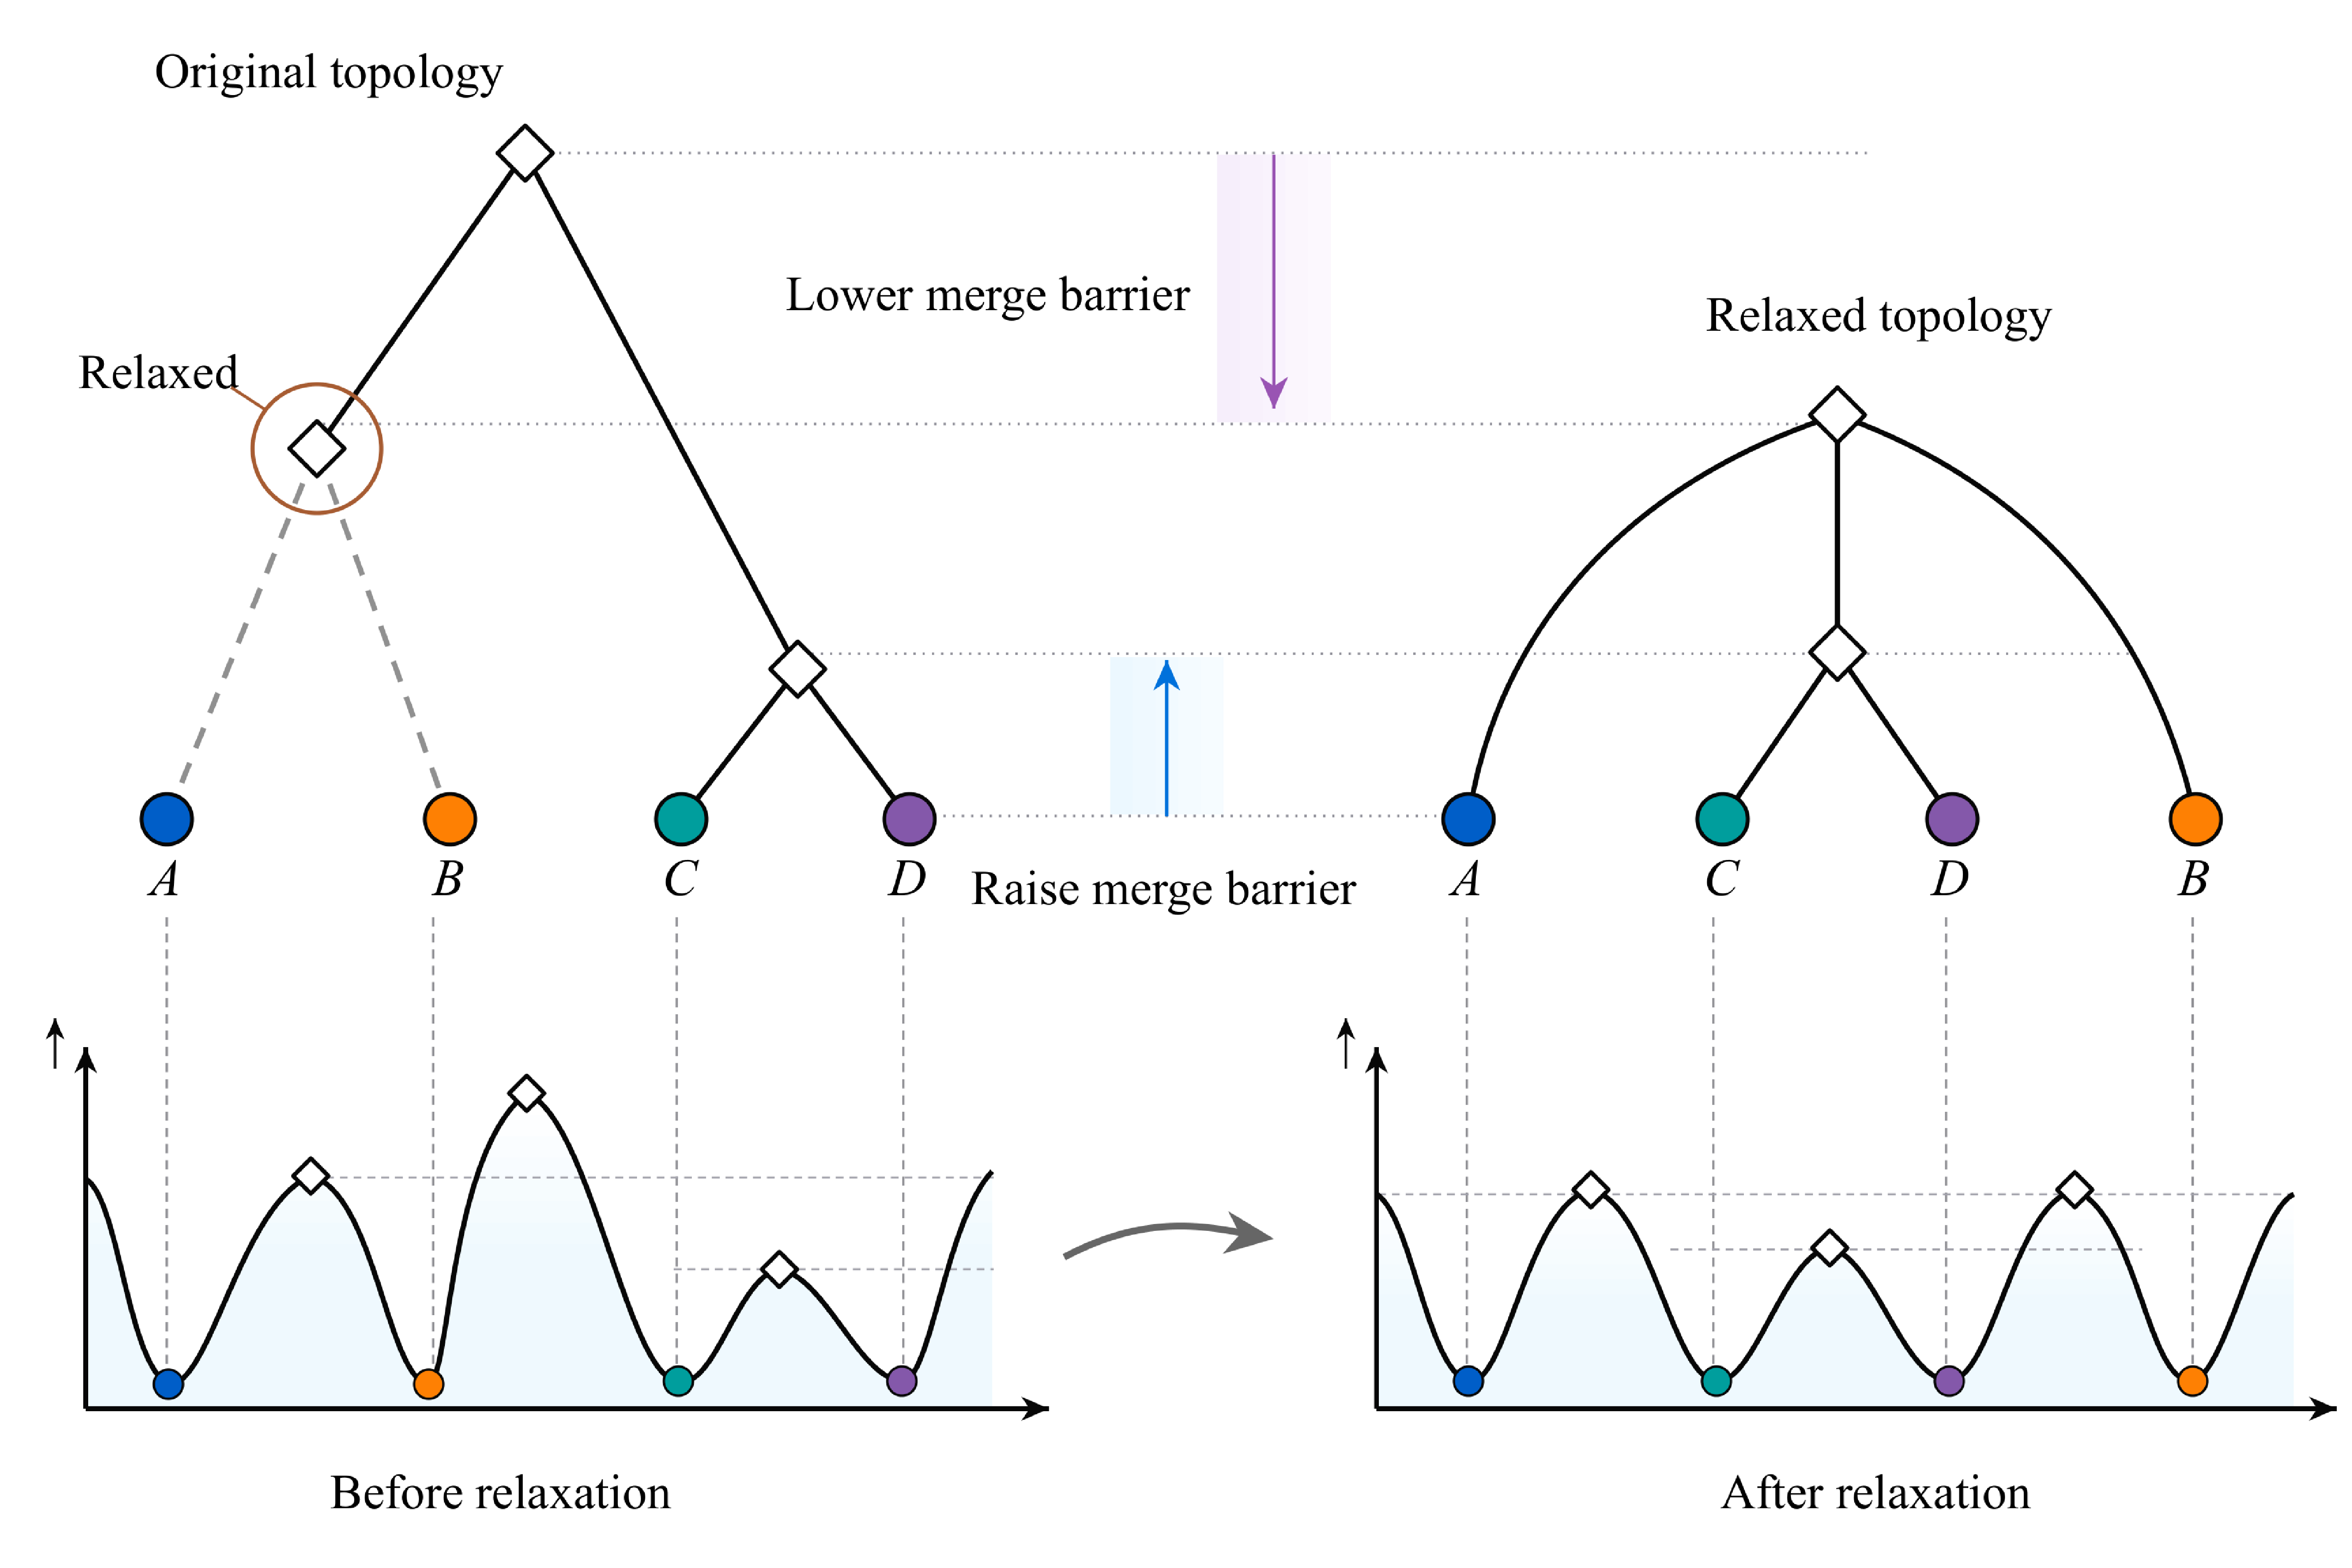
\includegraphics[width=\columnwidth]{../figures/anchor_relaxation_open.pdf}
\caption{Selective relaxation releases the $A,B$ block constraint and admits order $A,C,D,B$ while retaining the $C,D$ grouping. The accompanying profiles illustrate changed merge barriers; source-level guides show the hierarchy changes. Heights are schematic, and candidate orders still require evaluation against the original merge matrix.}
\label{fig:selective_relaxation}
\end{figure}
\subsection{Certified Position--Topology Bounds}\label{sec:bounds}
The construction can leave reference displacement even after optimization. The following bounds explain what topology and finite widths make unavoidable: the first answers how much a tree-compatible point order must deviate, the second adds interval packing, and the third asks which restrictions survive a merge-error allowance. They are analytical benchmarks, not three execution stages or search-pruning rules; construction uses the exact fixed-order costs $\tau$ and $\delta^*$. The resulting certificates apply independently of the layout algorithm. Full proofs and computational definitions accompany the paper in Supplementary Material. We suppress $t$ within a frame, use $[v]^+=\max(v,0)$, and take empty maxima as zero.

\subsubsection{Exact-Topology Reference-Order Bound}
For a reduced tree with strictly increasing proper-ancestor levels, exact topology makes every subtree contiguous. Let $[m_X,M_X]$ be the reference hull of the leaves in subtree $X$.
\begin{theorem}[Exact-Topology Position Bound]\label{thm:order}
Every zero-error profile has $\nroe(\pi)\ge\nu^*(T,q)$, where
\begin{equation}\label{eq:nu}
 \nu^*(T,q)=\frac{1}{2L}\max_v\max_{\substack{X,Y\in\mathrm{ch}(v)\\X\ne Y}}
 [\min(M_X-m_Y,M_Y-m_X)]^+.
\end{equation}
Recursive child ordering by reference-hull midpoint attains this point-model order bound in $O(n\log n)$ time.
\end{theorem}
\begin{proof}[Proof sketch]
Sibling blocks must choose one orientation. Their two possible inversion costs are $[M_X-m_Y]^+/2$ and $[M_Y-m_X]^+/2$. Midpoint order chooses the smaller; every inverted leaf pair is separated by sibling blocks at its LCA.
\end{proof}
The maximizing node and sibling pair say where the cost arises, at the merge of two subtrees whose projected ranges overlap, and the value says how much: half the overlap that remains in the cheaper orientation. Midpoint ordering attains the point-order optimum; finite intervals introduce additional constraints, considered next.

\subsubsection{Width-Aware Position Bound}
Finite widths, minimum gaps, anchor slack and canvas capacity add packing costs to the point-order obstruction. For a nonempty leaf set $S$, let $H_i=\rho W_i/2$, $\ell_i=q_i-W_i/2-H_i$, $h_i=q_i+W_i/2+H_i$, and $s_i=W_i+g$. Define two packing summaries:
\begin{equation}\label{eq:packing}
\begin{aligned}
 A(S)&=\max_{a\in S}\left(\ell_a+\sum_{\substack{i\in S\\\ell_i\ge\ell_a}}s_i\right),\\
 B(S)&=\max_{b\in S}\left(\sum_{\substack{i\in S\\h_i\le h_b}}s_i-h_b\right).
\end{aligned}
\end{equation}
The first uses upper reference-endpoint sets and the second lower sets; sorting and cumulative sums evaluate them. For disjoint leaf sets $X,Y$ and the full leaf set $\mathcal{F}$, write
\begin{equation}\label{eq:packingcost}
\begin{aligned}
 \omega(X,Y)&=\tfrac12\min\{A(X)+B(Y),A(Y)+B(X)\}-\tfrac g2,\\
 E_\partial&=\max\{0,B(\mathcal{F})-g,A(\mathcal{F})-g-L\}.
\end{aligned}
\end{equation}
Here $\omega$ takes the cheaper block orientation and $E_\partial$ accounts for both canvas ends. Let $\mathcal{P}_0$ contain every pair of distinct sibling descendant-leaf sets. The certificate is
\begin{equation}\label{eq:bwdef}
 \mathcal{B}_w(T,q,W)=\max\{E_\partial,\max_{(X,Y)\in\mathcal{P}_0}\omega(X,Y)\}.
\end{equation}
The dependence on $g$, $\rho$ and $L$ is through Eqs.~\ref{eq:packing}--\ref{eq:packingcost}; it is suppressed in the certificate's arguments.
\begin{theorem}[Width-Aware Position Bound]\label{thm:width}
For any feasible exact-topology interval layout,
\begin{equation}\label{eq:widthbound}
 \|x-q\|_\infty\ge\tau(\pi)\ge\mathcal{B}_w(T,q,W).
\end{equation}
With zero widths and gaps, $\mathcal{B}_w=L\nu^*(T,q)$.
\end{theorem}
\begin{proof}[Proof sketch]
The first and last anchors of selected leaves must enclose their intervals and intervening gaps, up to the allowed anchor slack. Upper and lower sets in Eq.~\ref{eq:packing} maximize the resulting shortfall against reference separation. Exact topology requires one orientation of every sibling pair; the canvas ends give the two one-sided costs.
\end{proof}
Thus $\mathcal{B}_w$ bounds all exact-topology legal interval orders and need not be attained; $\tau(\pi)$ is the attained minimum for a specified order. These quantities have coordinate units, whereas NROE and $\nu^*$ are normalized by $L$.

\begin{table}[!ht]
\centering
\caption{Balanced-mode parameter settings and runtime (seconds).}
\label{tab:anchor-parameters-final}
\footnotesize
\setlength{\tabcolsep}{2pt}
\renewcommand{\arraystretch}{0.95}
\begin{tabular}{@{}lcccc@{}}
\toprule
Parameter & Gaussian & Ring & Wildfires & Storms \\
\midrule
$\varepsilon$ & 1\% & 1\% & 5\% & 10\% \\
$L$ & 4096 & 196 & 4096 & 4096 \\
$s_w$ & 0.00581 & 0.00328 & 0.00053 & 0.01170 \\
$t_{opt}$ & 0.156 & 0.150 & 3.324 & 2.600 \\
$t_{total}$ & 1.340 & 0.486 & 4.424 & 63.447 \\
\bottomrule
\end{tabular}
\vspace{2pt}
\begin{minipage}{0.94\columnwidth}\footnotesize Weights $(4,1,0.5,0.1)$ and $\rho=0.5$ are fixed. $s_w$ is width per support measure; $L$ is raster length. Times are one run on Apple M4: optimization and full pipeline, respectively.\end{minipage}
\end{table}

\definecolor{pubgray}{gray}{0.45}
\begin{table*}[t]
\centering
\caption{Four-dataset comparison. Bold/underline mark the best/second distinct local measurements per dataset; ties share emphasis. Curves use fixed default orientations.}
\label{tab:quantitative-final}
\footnotesize
\setlength{\tabcolsep}{1.5pt}
\renewcommand{\arraystretch}{0.85}
\begin{tabular*}{\textwidth}{@{\extracolsep{\fill}}l*{12}{c}lccc@{}}
\toprule
\multirow{2}{*}{Dataset} & \multicolumn{3}{c}{Hilbert} & \multicolumn{3}{c}{Morton} & \multicolumn{3}{c}{TMTM} & \multicolumn{3}{c}{ST-MTM} & \multicolumn{4}{c}{Anchored (ours)} \\
\cmidrule(lr){2-4}\cmidrule(lr){5-7}\cmidrule(lr){8-10}\cmidrule(lr){11-13}\cmidrule(lr){14-17}
 & SNS$\downarrow$ & TW$\uparrow$ & NPE$\downarrow$ & SNS$\downarrow$ & TW$\uparrow$ & NPE$\downarrow$ & SNS$^\dagger$ & TW$^\dagger$ & NPE$\downarrow$ & SNS$^\dagger$ & TW$^\dagger$ & NPE$\downarrow$ & Mode & SNS$\downarrow$ & TW$\uparrow$ & NPE$\downarrow$ \\
\midrule
\multirow{2}{*}{Gaussian} & \multirow{2}{*}{$0.1117$} & \multirow{2}{*}{$0.6719$} & \multirow{2}{*}{$0.7557$} & \multirow{2}{*}{$\underline{0.0393}$} & \multirow{2}{*}{$\underline{0.8333}$} & \multirow{2}{*}{$0.7359$} & \multirow{2}{*}{\textcolor{pubgray}{$0.2500$}} & \multirow{2}{*}{\textcolor{pubgray}{$0.7700$}} & \multirow{2}{*}{$\underline{0.1118}$} & \multirow{2}{*}{\textcolor{pubgray}{$0.0600$}} & \multirow{2}{*}{\textcolor{pubgray}{$1.0000$}} & \multirow{2}{*}{$0.1154$} & Exact & $\mathbf{0.0353}$ & $\mathbf{0.9323}$ & $\mathbf{0.0089}$ \\
 &  &  &  &  &  &  &  &  &  &  &  &  & Balanced & $\mathbf{0.0353}$ & $\mathbf{0.9323}$ & $\mathbf{0.0089}$ \\
\multirow{2}{*}{Ring} & \multirow{2}{*}{$\mathbf{0.1252}$} & \multirow{2}{*}{$\mathbf{0.9048}$} & \multirow{2}{*}{$0.5941$} & \multirow{2}{*}{$0.1489$} & \multirow{2}{*}{$0.7619$} & \multirow{2}{*}{$0.6033$} & \multirow{2}{*}{\textcolor{pubgray}{$0.2800$}} & \multirow{2}{*}{\textcolor{pubgray}{$0.6800$}} & \multirow{2}{*}{$0.1756$} & \multirow{2}{*}{\textcolor{pubgray}{$0.2100$}} & \multirow{2}{*}{\textcolor{pubgray}{$0.8800$}} & \multirow{2}{*}{$0.2463$} & Exact & $0.1485$ & $\underline{0.8571}$ & $\underline{0.0471}$ \\
 &  &  &  &  &  &  &  &  &  &  &  &  & Balanced & $\underline{0.1334}$ & $\underline{0.8571}$ & $\mathbf{0.0395}$ \\
\multirow{2}{*}{Wildfires} & \multirow{2}{*}{$0.1883$} & \multirow{2}{*}{$0.8303$} & \multirow{2}{*}{$0.3641$} & \multirow{2}{*}{$0.1304$} & \multirow{2}{*}{$0.8758$} & \multirow{2}{*}{$0.1560$} & \multirow{2}{*}{\textcolor{pubgray}{$0.4400$}} & \multirow{2}{*}{\textcolor{pubgray}{$0.8800$}} & \multirow{2}{*}{$0.2280$} & \multirow{2}{*}{\textcolor{pubgray}{$0.2400$}} & \multirow{2}{*}{\textcolor{pubgray}{$0.9100$}} & \multirow{2}{*}{$0.3180$} & Exact & $\mathbf{0.0426}$ & $\mathbf{0.9136}$ & $\underline{0.0131}$ \\
 &  &  &  &  &  &  &  &  &  &  &  &  & Balanced & $\underline{0.0447}$ & $\underline{0.8989}$ & $\mathbf{0.0116}$ \\
\multirow{2}{*}{Storms} & \multirow{2}{*}{$0.1290$} & \multirow{2}{*}{$0.7403$} & \multirow{2}{*}{$0.3705$} & \multirow{2}{*}{$0.1180$} & \multirow{2}{*}{$0.7251$} & \multirow{2}{*}{$0.3468$} & \multirow{2}{*}{\textcolor{pubgray}{$0.3400$}} & \multirow{2}{*}{\textcolor{pubgray}{$0.7100$}} & \multirow{2}{*}{$0.5753$} & \multirow{2}{*}{\textcolor{pubgray}{$0.2100$}} & \multirow{2}{*}{\textcolor{pubgray}{$0.9400$}} & \multirow{2}{*}{$0.4579$} & Exact & $\underline{0.0790}$ & $\underline{0.8463}$ & $\underline{0.0399}$ \\
 &  &  &  &  &  &  &  &  &  &  &  &  & Balanced & $\mathbf{0.0743}$ & $\mathbf{0.8766}$ & $\mathbf{0.0140}$ \\
\bottomrule
\end{tabular*}
\vspace{2pt}
\begin{minipage}{\textwidth}\footnotesize $^\dagger$Grey: published TMTM/ST-MTM Temporal SNS/TW (ST-MTM Table~1, authors' inputs), shown for reference and excluded from emphasis; other entries are local measurements on the same inputs. Author inputs and coverage are unconfirmed. Local TW coverage (Gaussian/Ring/Wildfires/Storms) is 64/64, 1/40, 4/32, 11/744; ineligible frames are omitted. Published TW has two-decimal precision. Mode applies only to the anchored maps.\end{minipage}
\end{table*}

\subsubsection{Bounded-Topology Position Bound}
A merge-level allowance can release some contiguous blocks, but still limits interleaving. If leaf $k$ lies between descendants $i,j$ of node $u$, interval containment gives $V_{ik}^{\psi}\le V_{ij}^{\psi}$, hence $V_{ik}\le h(u)+2\eta$. Define $A_\eta(u)$ as the highest ancestor, including $u$, with $h(A_\eta(u))-h(u)\le2\eta$. This uses the accumulated ancestor-height difference in scalar units, on the reduced equal-level tree with the fixed labels of Eq.~\ref{eq:dtop}.

Let $\mathcal{P}_\eta$ consist of two types of leaf-set pairs: $(\mathcal{D}(u),\{k\})$ for every internal node $u$ and leaf $k\notin\mathcal{D}(A_\eta(u))$; and $(\mathcal{D}(u),\mathcal{D}(w))$ for internal nodes $u,w$ satisfying
\begin{equation}\label{eq:separatedpairs}
\begin{aligned}
 \mathcal{D}(w)\cap\mathcal{D}(A_\eta(u))&=\varnothing,\\
 \mathcal{D}(u)\cap\mathcal{D}(A_\eta(w))&=\varnothing.
\end{aligned}
\end{equation}
For any nonempty leaf set $X$, use its reference hull $[m_X,M_X]$ and define $\kappa(X,Y)=[\min(M_X-m_Y,M_Y-m_X)]^+/(2L)$. The two certificates are
\begin{equation}\label{eq:chaindef}
\begin{aligned}
 C_\eta(T,q)&=\max_{(X,Y)\in\mathcal{P}_\eta}\kappa(X,Y),\\
 C_{w,\eta}(T,q,W)&=\max\{E_\partial,\max_{(X,Y)\in\mathcal{P}_\eta}\omega(X,Y)\}.
\end{aligned}
\end{equation}
\begin{theorem}[Bounded-Topology Position Bound]\label{thm:chain}
In a profile with $\dtop\le\eta$, no leaf outside $\mathcal{D}(A_\eta(u))$ can lie between two leaves of $u$. Every pair in $\mathcal{P}_\eta$ lies wholly in one block orientation or the other. Consequently,
\begin{equation}\label{eq:chainbounds}
 \nroe(\pi)\ge C_\eta(T,q),\qquad
 \tau(\pi)\ge C_{w,\eta}(T,q,W),
\end{equation}
with the second inequality applying to the interval model.
\end{theorem}
The separation principle excludes interleaving for each eligible pair; the two possible orientations then yield $\kappa$ and $\omega$. Thus $C_\eta$ bounds normalized reference-order error, while $C_{w,\eta}$ includes finite-width and boundary costs in coordinate units. Flattening every parent gap of at most $2\eta$ gives a second valid certificate; neither dominates, since flattening also separates single-leaf pairs that $\mathcal{P}_\eta$ omits, and we report the larger. The pair set also says what releases a conflict: a subtree may interleave with its sibling once $2\eta$ reaches the gap between its own merge level and its parent's, so conflicts at deep merges stay expensive.

The allowance concerns the displayed hierarchy; the source field and feature identities stay fixed. A larger feasible set need not improve every feature or every heuristic result. These bounds are reported as benchmarks for unavoidable error; ranking and continuous acceptance use the exact fixed-order evaluations in Section~\ref{sec:construction}. Continuous feasibility does not certify the full rendered raster.

\section{Experiments}\label{sec:experiments}
We evaluate whether anchoring improves absolute reference positioning, what topology relaxation changes, how accurate the position bounds are, and how the resulting maps support qualitative inspection. Four planar datasets provide the primary numerical evidence and two volumetric datasets add a local comparison with TMTM; the bounds are also tested on controlled trees and on the frames of an earlier benchmark. We distinguish published scores, local measurements and qualitative archives throughout.
\begin{table}[t]
\centering
\caption{Volumetric datasets and Balanced-mode parameter settings.}
\label{tab:volume-parameters}
\footnotesize
\setlength{\tabcolsep}{2pt}
\renewcommand{\arraystretch}{0.95}
\begin{tabular}{@{}lcc@{}}
\toprule
Parameter & Cylinder & Tangaroa \\
\midrule
Frames & 102 & 201 \\
Grid & $135\times64\times48$ & $300\times180\times120$ \\
Scalar & $Q$-criterion & Speed $\|\mathbf{v}\|$ \\
Persistence & 2\% per-frame range & 0.2 absolute \\
Reference & $+x$ & $+x$ \\
$\varepsilon$ & 1\% & 33.33\% \\
$L$ & 32768 & 131072 \\
$s_w$ & $2.70668\times10^{-5}$ & 0.40953 \\
Weights & $(0.1,16,0,0.1)$ & $(0,64,0,0)$ \\
$\rho$ & 1 & 1 \\
Gap$/L_{world}$ & $1/300$ & $1/960$ \\
Extra$/L_{world}$ & 0.1 & 0.1 \\
\bottomrule
\end{tabular}
\vspace{2pt}
\begin{minipage}{0.94\columnwidth}\footnotesize Weights are reference, geometry, temporal and eccentricity. $s_w$ is width per support measure (Cylinder voxel counts; Tangaroa physical volume); $L$ is raster length, distinct from the physical canvas extent $L_{world}$. Exact uses zero allowance with the same other parameters as its Balanced counterpart.\end{minipage}
\end{table}

\subsection{Datasets and Evaluation Protocol}
Our four planar inputs are Gaussian, Ring, Wildfires and Storms (64, 40, 32 and 744 frames). Raster lengths are 4096, except Ring's original 196 positions. The ST-MTM persistence numbers are tested as per-frame range fractions $p=(0.001,0.001,0.15,0.105)$, or $0.1\%,0.1\%,15\%,10.5\%$; all 880 thresholds were checked~\cite{STMTM:2026}. Gaussian is a three-peak reconstruction, Ring uses the archived generator, Wildfires aggregates FRP into 32 grids, and Storms uses ERA5 anomalies with the archived moving-mean and smoothing convention. Author-processed arrays are unavailable, so these are disclosed local reconstructions, not identical-input reproductions.

The volumetric inputs are Cylinder (102 frames, $135\times64\times48$, $Q$-criterion)~\cite{Camarri:2005:Cylinder,Weinkauf:SquareCylinder} and Tangaroa (201 frames, $300\times180\times120$, velocity magnitude)~\cite{Popinet:2004:Tangaroa}. Cylinder computes $Q$ from the original $192\times64\times48$ velocity grids before cropping; 2\% persistence uses each frame's scalar range, followed by one fixed sequence scaling of $-Q$. Tangaroa uses speed clipped to $[0,2]$, replaces near-zero values below $10^{-6}$ by the archived inflow value 1, and retains absolute persistence 0.2. These preprocessing choices are shared with the local TMTM adapter. Cylinder's 102-frame subset differs from the 508 frames reported in the first paper; no author-score reproduction is claimed.

For the volumetric comparison, the reference is restricted to the positive Cartesian axes rather than the continuous direction in Section~\ref{sec:construction}. The archived offline rule chooses the axis capturing the most squared displacement of matched support centroids, with a minimum-image correction for Cylinder's periodic $z$ coordinate (period 6); both datasets select $+x$. Centroids select the axis only: placement targets remain leaf extrema projected onto that fixed axis and full-domain range. This rule uses the full input sequence, not output SNS/TW/NPE, and does not define an independent test. The stored layout configurations are exploratory selections; Table~\ref{tab:volume-parameters} reports their different weights and budgets. In particular, Tangaroa's zero reference weight makes its configuration geometry-dominated; low measured NPE is an outcome, not evidence that an absolute-reference penalty caused it.

Within each local dataset, methods share source trees, identities and geometry inputs, and NPE uses one common offline extremum reference and projected range. SNS measures squared scale-normalized stress between support-centroid and anchor distances~\cite{Smelser:2025:Scale,STMTM:2026}; TW measures neighborhoods~\cite{Venna:2001:NP}, with $k=(1,3,5,3)$ and $0<k<n_t/2$. Ineligible frames are omitted. Absolute anchoring uses
\begin{equation}\label{eq:experimental-npe}
\mathrm{NPE}=\frac{1}{T}\sum_t\frac{\max_i|x_i^t-q_i^t|}{L_{world}}.
\end{equation}
TMTM/ST-MTM SNS/TW are quoted from ST-MTM Table~1 (Temporal mode); their NPE is measured with local adapters and shared references, each mirrored once if its first multi-leaf frame correlates negatively with the reference. Table~\ref{tab:quantitative-final} distinguishes these sources. Local TW coverage is 64/64, 1/40, 4/32 and 11/744; author coverage is unspecified.

Hilbert and Morton provide sample-domain baselines~\cite{Franke:2021:1DP}. Their grid orientation is fixed ($x$ columns, $y$ rows), with no rotation, reflection or reversal search. Curves use power-of-two padding, discard out-of-domain samples, and map each extremum's full-grid rank to the common canvas at the original raster length. They impose neither merge-tree topology nor finite-width constraints.

\begin{figure*}[t]
\centering
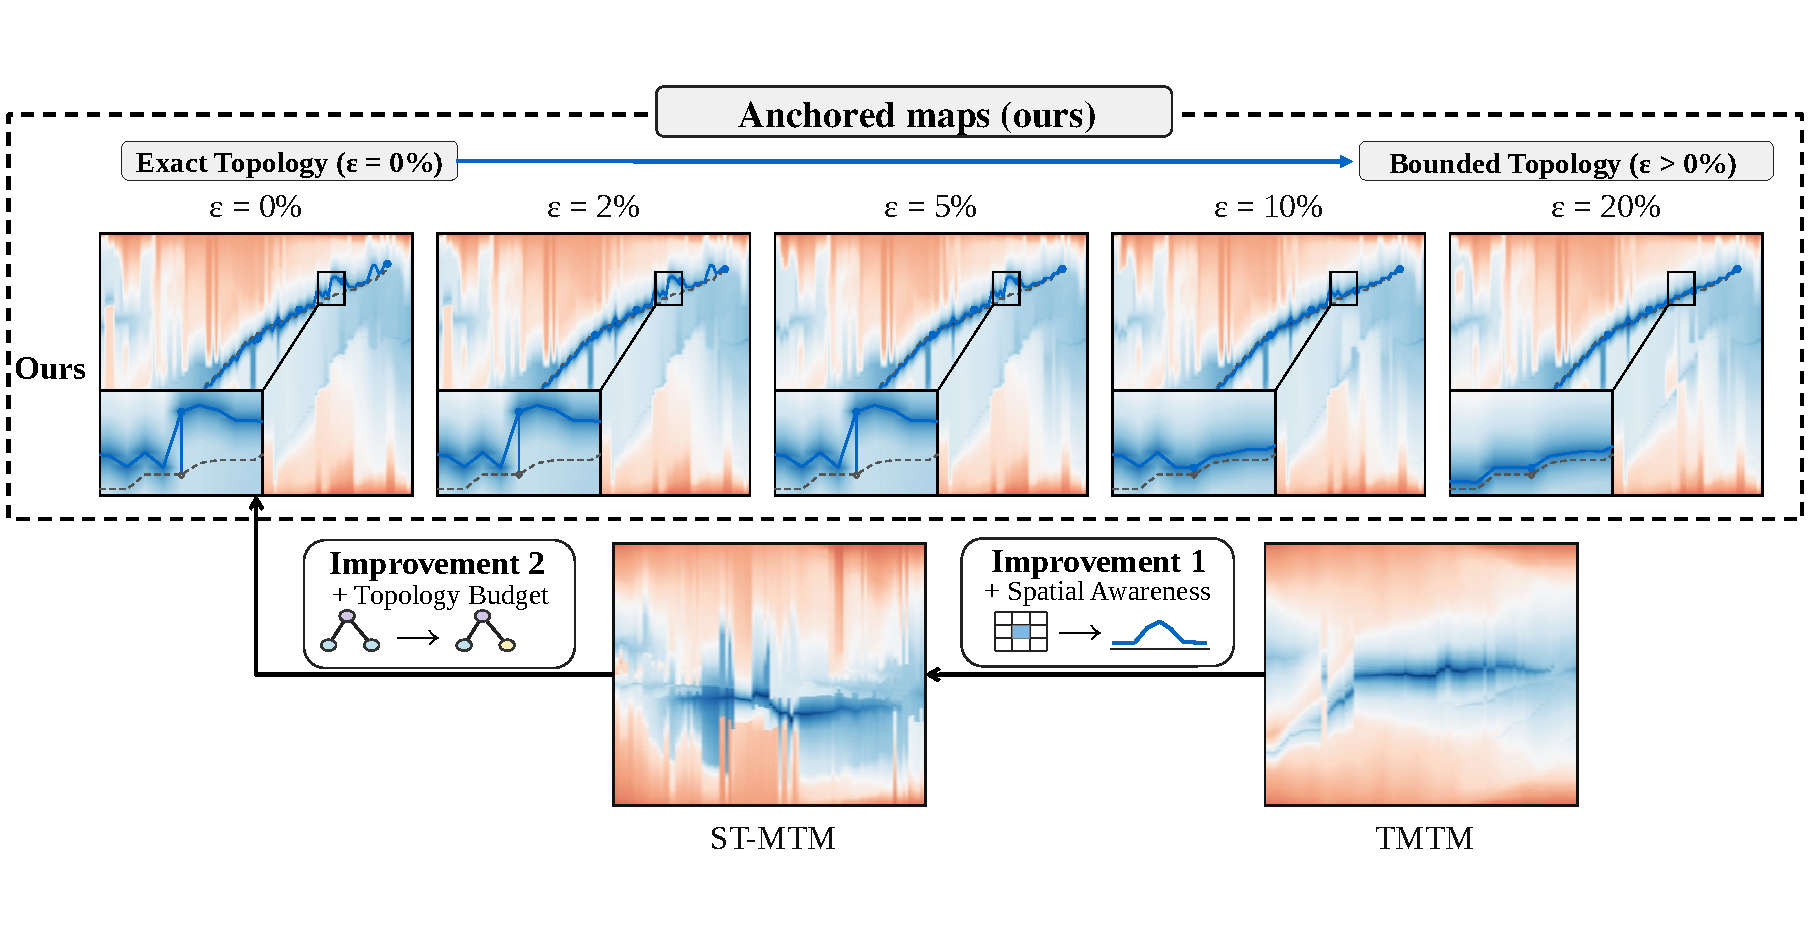
\includegraphics[width=\textwidth]{../figures/anchor_storms_budget_maps_v17.pdf}
\caption{Storms parameter maps and method comparison. Anchored maps span exact topology ($\varepsilon=0$) and bounded topology (2, 5, 10 and 20\%), with the original trajectories and common local crops. TMTM and ST-MTM maps use the same scalar fields and augmented trees through local implementations. Spatial awareness and topology budget indicate the respective conceptual improvements. All maps show frames 355--460 with the original blue--orange scale, $[-35,35]$ hPa. Module connections summarize design differences rather than exact algebraic equivalence; multiway-tree adapters are disclosed in the text.}
\label{fig:storms-budget-profiles}
\end{figure*}
\begin{figure}[!t]
\centering
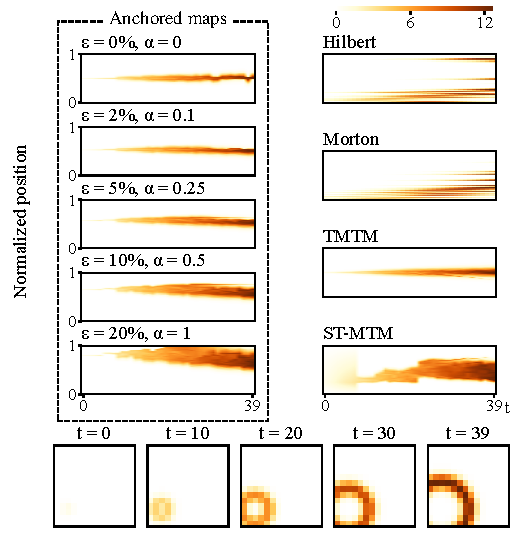
\includegraphics[width=\columnwidth]{../figures/anchor_ring_result_v17.pdf}
\caption{Ring comparison. Left: anchored maps with topology allowance $\varepsilon$ and guidance strength $\alpha=\varepsilon/20\%$ raised together, from neutral central targets ($\alpha=0$) to full spatial guidance ($\alpha=1$); the upward shift reflects guidance, not the allowance alone. Right: supplied Hilbert/Morton reference panels and same-input local TMTM/ST-MTM results. Below: source snapshots at frames 0, 10, 20, 30 and 39. All computed maps use 40 frames and 196 positions; the scalar key applies to computed maps and snapshots. Vertical coordinates denote normalized layout position or curve rank.}
\label{fig:ring-result}
\end{figure}

\paragraph{Mode selection.}
For the four planar datasets, Exact uses $\varepsilon=0$. Balanced selects a positive budget from 1--10\% (1\% steps) on the first chronological quarter. Among legal reconstructions with attained NMLE$_{\max}\le\varepsilon$, it minimizes
\begin{equation}\label{eq:balanced-validation-score}
J=0.5\,\mathrm{NPE}_{norm}+0.5\,\mathrm{SNS}_{norm}.
\end{equation}
Terms are min--max normalized over legal candidates; constant terms contribute zero. Within 0.01 of the minimum, smaller budgets then attained errors break ties. Budgets are frozen before full runs, without a zero-budget fallback. Full results include validation frames; earlier outputs were observed, so this is not a new blind test.




\subsection{Reference Positioning and Spatial Quality}

ST-MTM reports higher TW than the anchored maps on all four inputs. Its published SNS values are higher than our local ones, but they come from the authors' inputs and frame coverage, so we do not rank SNS or TW across these sources; Wildfires Exact's TW of 0.9136 is also too close to the published two-decimal 0.91 to establish an advantage.

Against fixed Hilbert and Morton curves, Balanced improves SNS and TW on Gaussian, Wildfires and Storms. Ring is an exception: Hilbert achieves SNS 0.1252 and TW 0.9048, versus Balanced's 0.1334 and 0.8571; its TW evidence covers only one eligible frame. Balanced has lower NPE than both curves and both merge-tree adapters on every input. Reductions relative to the ST-MTM adapter are 92.3\%, 84.0\%, 96.3\% and 96.9\%. This supports alignment to the specified reference, not general visualization quality: traversal coordinates need not represent a physical projection, and relative geometry does not determine an absolute origin.

\subsection{Volumetric Comparison with TMTM}
\begin{table}[t]
\centering
\caption{Volumetric comparison with a fixed $x$ reference. Bold/underline mark best/second distinct values per dataset; ties share emphasis.}
\label{tab:volume-comparison}
\footnotesize
\setlength{\tabcolsep}{1.2pt}
\renewcommand{\arraystretch}{0.9}
\begin{tabular*}{\columnwidth}{@{\extracolsep{\fill}}lccc lccc@{}}
\toprule
\multirow{2}{*}{Dataset} & \multicolumn{3}{c}{TMTM} & \multicolumn{4}{c}{Anchored (ours)} \\
\cmidrule(lr){2-4}\cmidrule(lr){5-8}
 & SNS$\downarrow$ & TW$\uparrow$ & NPE$\downarrow$ & Mode & SNS$\downarrow$ & TW$\uparrow$ & NPE$\downarrow$ \\
\midrule
\multirow{2}{*}{Cylinder} & \multirow{2}{*}{$0.2956$} & \multirow{2}{*}{$\underline{0.8017}$} & \multirow{2}{*}{$0.4769$} & Exact & $\underline{0.1226}$ & $0.8010$ & $\underline{0.1773}$ \\
 &  &  &  & Balanced & $\mathbf{0.0329}$ & $\mathbf{0.9117}$ & $\mathbf{0.0458}$ \\
\multirow{2}{*}{Tangaroa} & \multirow{2}{*}{$0.5255$} & \multirow{2}{*}{$0.6701$} & \multirow{2}{*}{$0.3866$} & Exact & $\underline{0.1204}$ & $\underline{0.8213}$ & $\underline{0.1285}$ \\
 &  &  &  & Balanced & $\mathbf{0.1124}$ & $\mathbf{0.8408}$ & $\mathbf{0.0653}$ \\
\bottomrule
\end{tabular*}
\vspace{2pt}
\begin{minipage}{\columnwidth}\footnotesize All values are local measurements, including adapted TMTM. TW uses $k=1$, with coverage 102/102 and 201/201. Mode applies only to the anchored maps. Configurations are frozen exploratory results, not a blind test; settings appear in Table~\ref{tab:volume-parameters}.\end{minipage}
\end{table}

Table~\ref{tab:volume-comparison} follows the planar table's metric order and Exact--Balanced grouping, but compares only with locally adapted TMTM. All three metrics are recomputed over the complete sequences; SNS uses three-dimensional support-centroid distances, TW uses $k=1$ with full frame coverage, and NPE uses extremum targets along the common $x$ axis. Balanced has lower SNS and NPE and higher TW than TMTM on both datasets. Exact and Balanced share the same axis, trees, retained leaf identities and layout weights; only the merge allowance differs. Exact has zero measured fixed-leaf merge error, and both stored Balanced runs pass their declared topology budgets. The large Tangaroa allowance (33.33\%) and its geometry-dominated objective limit attribution: these are selected configurations, not evidence of universal superiority or a controlled comparison with planar default weights.

\subsection{Topology Validity and the Effect of Relaxation}
Exact has zero fixed-leaf merge-matrix error. Balanced attains maximum NMLE of 0, 0.982\%, 4.421\% and 9.985\%, within its allowances; all eight runs pass continuous and raster checks without collapsed anchors. Checks include diagonal extrema, not every augmented internal label. Ring requires checked joint integer rounding in 26 Exact and 21 Balanced frames, retaining its 196 positions and continuous order.

Balanced reduces NPE relative to Exact by 16.2\% on Ring, 11.6\% on Wildfires and 64.9\% on Storms. Gaussian is unchanged despite its positive 1\% budget. SNS improves on Ring and Storms but rises from 0.0426 to 0.0447 on Wildfires. Budget relaxation therefore does not improve every metric.

These Exact--Balanced comparisons measure the effect of the selected allowances, rather than a component ablation. A positive allowance need not change the selected order or improve reference positioning. The budget constrains merge-level error; it is not a direct bound on spatial displacement.

\subsection{Accuracy of the Position Bounds}\label{sec:bounds-eval}
\begin{figure}[t]
\centering
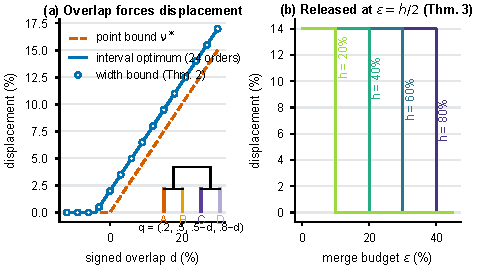
\includegraphics[width=\columnwidth]{../figures/anchor_controlled_bounds.pdf}
\caption{Controlled four-leaf trees (inset: sibling pairs and references). (a) Increasing sibling-range overlap $d$ forces displacement; the width bound of Theorem~\ref{thm:width} (circles) equals the optimum over all 24 leaf orders. (b) At $d=24\%$, the 14\% displacement disappears exactly when the merge budget reaches half the parent gap $h$, for all four gaps, as Theorem~\ref{thm:chain} predicts. Percentages refer to a unit canvas or a unit scalar range.}
\label{fig:controlled}
\end{figure}
\emph{Controlled trees.} To separate the causes of displacement, we fix two sibling pairs $\{A,B\}$ and $\{C,D\}$ that merge at $0.4$ below a root at $1$, with leaf values $0$ and references $(0.2,0.5,0.5-d,0.8-d)$ on a unit canvas, and vary the signed overlap $d$ from $-0.12$ to $0.30$. Across 43 overlaps and four widths, we compare the bounds with all 24 leaf orders, each placed by an independent minimax LP. Topology alone forces exactly $\nu^*=\max(0,d)/2$. With widths $0.06$, gap $0.01$ and $\rho=0.5$, the width bound, our search and the exhaustive optimum coincide at $\tau=\max(0,(d+0.04)/2)$ (Fig.~\ref{fig:controlled}a): 12\% for points and 14\% for intervals at $d=0.24$. A merge allowance removes the conflict exactly where Theorem~\ref{thm:chain} admits interleaving, at $2\varepsilon=h$ for all four parent gaps $h$ tested (Fig.~\ref{fig:controlled}b).

\emph{Real trees.} We also evaluate the bounds on the frames of an earlier benchmark with one default configuration (Supplementary Material): five planar sequences with 614 frames, namely 12-hourly ERA5 sea-level pressure~\cite{Hersbach:2020:ERA5}, daily wildfire radiative power~\cite{Franke:2021:1DP}, outgoing longwave radiation~\cite{NOAA:OLR}, PM$_{2.5}$ concentration~\cite{Dong:2026:PM25} and Ring, and the Tangaroa and Cylinder volumes. In Exact Mode, the interval cost $\tau$ of the selected order equals $\mathcal{B}_w$ on 606 of the 614 planar frames, so on these frames no exact-topology order has a smaller worst displacement; at $\varepsilon=10\%$ the bounded-topology certificate is met on 596. Volumetric trees are harder: the bound is met on 81 of 102 Cylinder and 27 of 201 Tangaroa frames, and the remaining gap may lie in the bound or in the search. Because Theorem~\ref{thm:order} needs no layout, it also measures existing maps: midpoint ordering attains $\nu^*$ on the same tree, so order error above $\nu^*$ is chosen by the order rule rather than forced by the hierarchy. On these seven sequences, 53--95\% of the order error of TMTM and 31--95\% of that of ST-MTM lies above $\nu^*$, each evaluated in the mirror that agrees better with the reference. Supplementary Fig.~S1 places all maps against the bounds. Relaxation buys position where conflicting subtrees merge just below their parent: 1\% halves the forced order error on Wildfires (5.80\% to 2.77\%), whereas on Tangaroa the bound stays above 7\% up to $\varepsilon=5\%$. Over 400 reference directions, the mean order bound spans 4.70--10.14\% on Tangaroa and 5.49--28.15\% on Cylinder, computed before any map is drawn (Supplementary Fig.~S2).

\subsection{Ring Case Study: Temporal Overview and Source Snapshots}

Figure~\ref{fig:ring-result} shows a joint guidance--topology sweep on Ring: $\varepsilon=0,2,5,10,20\%$ and guidance strength $\alpha=\varepsilon/20\%$. Layout targets interpolate between the canvas midpoint and the fixed $-128.7^\circ$ physical projection: $q_{layout}=(1-\alpha)q_{mid}+\alpha q_{physical}$. Thus stronger guidance moves the reconstructed ring upward through actual optimization, with no image translation. This qualitative sweep changes both guidance and topology allowance, and each panel lists both values; it is not an epsilon-only ablation, its $\alpha=0$ panel is not the Exact Mode of Table~\ref{tab:quantitative-final}, and it does not replace the frozen main-table settings. TMTM/ST-MTM maps use the same fields and trees; Hilbert/Morton remain supplied references. Five source snapshots show expansion and strengthening.

\subsection{Storms Case Study: Reading Budgeted Maps}

The upper row of Fig.~\ref{fig:storms-budget-profiles} retains the original five-budget qualitative Storms archive of Fig.~\ref{fig:storms_overview}, separate from main-table preprocessing. The 0, 2 and 5\% layouts overlap locally, while 10 and 20\% move the selected feature toward its fixed reference. The lower row shows TMTM and ST-MTM maps recomputed on these same 744 scalar fields and augmented trees, showing the same event window without per-panel recoloring or display translation. TMTM uses overlap-driven temporal subtree alignment in place of anchored placement; ST-MTM uses geometry-based ordering and distance-aware placement with temporal position constraints. The local TMTM implementation handles genuine multiway saddles with equal-level separator copies; the ST-MTM adapter refines them into a stable-ID equal-level binary hierarchy and checks the original leaf LCA matrices. Both baselines use start frame 40 and 8192-position display rasters. They are local implementations, not author binaries. The module arrows describe replacements and additions rather than claiming exact algorithmic reductions or changing the main-table protocol.

\subsection{Parameters and Computational Cost}
Table~\ref{tab:anchor-parameters-final} lists the four planar Balanced budgets (1, 1, 5 and 10\%) and layout parameters; Table~\ref{tab:volume-parameters} separately lists the volumetric datasets and settings. The planar table reports one uncached Balanced run on Apple M4, with one BLAS/TTK thread, sequential extraction and the default HiGHS scheduler. Optimization includes ordering and placement; total time additionally includes preprocessing, trees, matching/reference estimation, rasterization, I/O and checks. Imports, reporting and metric export are excluded; OS caches may be warm. Timings do not establish speedup significance. Baseline NPE uses the disclosed CompactTMTM and ST-MTM solver adaptations, not author binaries.

\section{Discussion and Limitations}
The bounds separate forced from chosen displacement. Order error above $\nu^*$ is always removable without changing the tree, since midpoint ordering attains $\nu^*$; the width-aware and bounded-topology bounds need not be attained, so an excess above them may lie in the bound rather than in the layout.

A fixed physical reference and a geometry-oriented embedding answer different questions. Anchored maps support reading positions along a chosen spatial coordinate; ST-MTM's higher reported TW highlights the value of preserving local neighborhoods. Neither property guarantees the other. The four-input results therefore support a task-specific anchoring claim, rather than universal superiority in spatial or temporal fidelity.

The empirical comparison has three limitations. First, author-processed fields and their small-sample TW protocol are not fully available, so published SNS/TW cannot provide an identical-input significance test. Second, the reference and tracking are computed offline from the supplied sequence; support overlap is a correspondence proxy, not a physical-identity annotation. Third, order search is heuristic and a continuous certificate does not remove integer-rendering constraints. We check actual fixed-label merge matrices after reconstruction, but do not claim a certificate for every augmented internal label.

The experiments also do not establish perceptual readability, physical-motion judgment accuracy, repeated-run speedups or generalization to unseen datasets. These require separate studies. Keeping source provenance, coverage, failed candidates and attained topology errors alongside the numerical scores is necessary when extending this evaluation.
\section{Conclusion}
Keeping the merge tree on the axis of a temporal merge tree map has a positional price; three layout-independent bounds state the displacement that exact topology, finite widths and a bounded merge error force on any layout. The selected exact-topology order attains the width-aware bound on 606 of 614 planar frames, and 31--95\% of the order error of TMTM and ST-MTM is not forced by the tree. On four local inputs, anchored maps place features closer to their references than same-input baselines within every merge budget, while ST-MTM's published neighborhood preservation remains higher.
% Flush pending floats without forcing an otherwise empty bibliography page.
\FloatBarrier
\begingroup
\interlinepenalty=10000
\bibliographystyle{abbrv-doi-narrow}
\bibliography{../refs}
\endgroup
\end{document}
